\documentclass[journal,onecolumn]{IEEEtran}

\usepackage{cite}
\usepackage{amsmath,amssymb}
\usepackage{graphicx}
\usepackage{booktabs}
\usepackage{xcolor}
\usepackage{listings}
\usepackage{algorithm}
\usepackage{algpseudocode}
\usepackage{array}
\usepackage{multirow}
\usepackage{url}
\usepackage{float}

\graphicspath{{figures/}}

\lstset{
    basicstyle=\ttfamily\small,
    breaklines=true,
    columns=fullflexible,
    frame=single
}

\begin{document}

\title{Hybrid Quantum-Classical Machine Learning Framework for Web Attack Detection Using Burp Suite HTTP Traffic}

\author{
\IEEEauthorblockN{Anamika Bharti}
\IEEEauthorblockA{
Department of Computer Science \\
VIT Vellore, India \\
email@domain.com}
}

\maketitle

\begin{abstract}
As attacks on web applications continue to evolve in both scale and sophistication, attackers are increasingly relying on advanced obfuscation techniques to evade detection by traditional security mechanisms such as web application firewalls and signature-based intrusion detection systems. These obfuscation strategies often involve encoding payloads, manipulating syntax, and injecting structurally complex inputs that appear legitimate at first glance but are designed to exploit underlying system vulnerabilities.
In response to these challenges, this paper explores the design and development of an advanced hybrid detection framework that combines multiple complementary machine learning paradigms. The proposed approach integrates an anomaly-based detection model to identify deviations from normal traffic behavior, along with an ensemble classifier that leverages the strengths of multiple classical learning algorithms to improve robustness and reduce false positives. Additionally, the framework incorporates variational quantum classifiers, which are capable of capturing complex, non-linear relationships in high-dimensional feature spaces that may be difficult for classical models to represent effectively.
A key component of the proposed system is a confidence-gated decision mechanism. This mechanism evaluates the certainty of the classical ensemble output and dynamically routes low-confidence or suspicious instances to the quantum classifier for deeper and more precise analysis. By combining classical efficiency with quantum-enhanced expressiveness, the system aims to achieve higher detection accuracy, improved generalization, and stronger resilience against evolving and obfuscated attack patterns in modern web application environments.
\end{abstract}

\begin{IEEEkeywords}
Quantum Machine Learning, Variational Quantum Classifier (VQC), Web Application Security, Hybrid Intrusion Detection, Intrusion Detection System, Ensemble Learning, Obfuscated Attack Detection
\end{IEEEkeywords}

\begin{table}[h]
\centering
\caption{Summary of System Notations and Architectural Parameters}
\label{tab:notations}
\small
\setlength{\tabcolsep}{1 pt}
\begin{tabular}{|c|l|l|}
\hline
\textbf{Symbol} & \textbf{Parameter Definition} & \textbf{Operational Value/Setting} \\
\hline
$\tau$ & Escalation Threshold & 0.85 (Confidence Cut-off) \\
\hline
$H(S)$ & Shannon Entropy Score & Metric for payload randomness \\
\hline
$N_{qubit}$ & Quantum Circuit Scale & 4 Qubits (Simulated via PennyLane) \\
\hline
$D_{feat}$ & Input Dimensions & 26 (Reduced to 4 via PCA for VQC) \\
\hline
$\theta$ & Variational Parameters & Rotation angles ($R_y$, $R_z$) in Ansatz \\
\hline
$P_{acc}$ & Final System Accuracy & 100\% (Hybrid Performance) \\
\hline
\end{tabular}
\end{table}


% =========================
\section{Introduction}
Table~\ref{tab:notations} summarizes the key mathematical notations and architectural parameters used throughout this paper.

\subsection{Background}
These days, web apps shape how people talk, do business, move money, tap into clouds, and share huge amounts of information worldwide. Because companies now lean heavily on online systems to reach users quickly and widely, more doors are open for hackers to walk through. With growth comes danger - cyber dangers shift just as fast, sometimes faster, as bad players invent fresh tricks to dodge guards and slip inside weak spots built into software itself.

Year after year, the OWASP Top 10 points out serious flaws in today's web apps. Still topping the list are injection problems - like SQLi, CMDi, XSS - not going away because they're easy to pull off yet powerful enough to work on many systems. Though tools have improved, these issues keep showing up, version after version. Proof? They stick around simply because actual defenses often fall short. Even with progress, fixing them completely hasn't happened yet.

One way to handle these risks? Many companies now use Web Application Firewalls, placing them right at the front to stop harmful web traffic early. Instead of learning behaviors, older styles depend on fixed rules or detect matches to already-seen threats - sometimes allowing only what is recognized as safe, sometimes blocking clear dangers by name. These methods work fine when dealing with familiar attacks that follow predictable paths. Yet here's the catch - they simply miss the meaning hidden within cleverer requests aimed at breaking through.

So most old-style WAFs can't keep up when attacks change fast. Because of this gap, hackers now often use clever tricks meant to slip past fixed rule sets. Think: scrambling code with Base64 or URL methods just enough to look harmless. Sometimes they swap letters for hex or strange symbols so filters miss them. Other times they hide bad parts inside random notes slipped into database questions. Even the shape of the attack shifts - twisted around but still dangerous underneath. Often, layers pile on top - encoded again and again like wrapping paper over traps.

Most old-style firewalls do not grasp context or learn from changes. As a result, they struggle with scrambled data. These tools fall short when threats shift quickly in live environments. Because of this gap, smarter systems are emerging - ones that watch how actions unfold rather than just checking fixed rules. Understanding purpose and structure inside incoming information becomes key.

The evolution of SQL injection bypass techniques is summarized in Table~\ref{tab:sqli}.

\begin{table}[htbp]
\caption{Evolution of SQL Injection Bypass Techniques}
\label{tab:sqli}
\centering
\resizebox{\columnwidth}{!}{
\begin{tabular}{|c|c|c|c|}
\hline
\textbf{Gen} & \textbf{Technique} & \textbf{Description} & \textbf{WAF Limitation} \\
\hline
1st & URL Encoding & \%20, \%27 encoding & Easily decoded \\
\hline
2nd & Double Encoding & \%2527 encoding & Decoded once only \\
\hline
3rd & Comment Split & SEL/**/ECT & Signature breaks \\
\hline
4th & Tautologies & OR 1=1 logic & Infinite variations \\
\hline
5th & Polymorphic & Base64 + logic & Needs AI detection \\
\hline
\end{tabular}
}
\end{table}

The progression from simple encoding to polymorphic payloads highlights the growing limitations of traditional WAFs and motivates the need for adaptive detection mechanisms.

\subsection{Motivation}
Nowadays, older rule-driven defenses feel sluggish next to modern machine learning methods in spotting digital threats. Instead of just checking known code fingerprints, these new tools study vast amounts of activity to spot oddities. Where past models froze responses into fixed logic trees, today's ones adapt using probability clues hidden across datasets. Sudden shifts in user habits? They catch those now. Detection isn't about rigid checklists anymore but recognizing subtle echoes of harm through number trails.

Out of nowhere, tools like Random Forests and Gradient Boosting - XGBoost included - have gotten much better at spotting sneaky web app attacks. What makes them stand out is how they pick up patterns from huge sets of data pulled straight from network flows, HTTP headers, and request contents. Instead of just looking for fixed phrases or rigid rules, they study habits hidden in the numbers: trends, clusters, odd gaps. Because of this shift in approach, their guesses hold up even when attack styles change unexpectedly.

Even with their strengths, traditional machine learning methods struggle in settings that are constantly shifting and full of deliberate interference. A major hurdle arises from the limits of standard computers, which handle data using only ones and zeros. Because of this rigid format, these systems often fail to capture intricate patterns in massive datasets. When adversaries craft inputs meant to slip past defenses, the shortcoming becomes even more pronounced.

Sometimes, attackers design fake data that looks normal but hides harmful actions inside slight changes to features. Because of these small shifts, regular machine learning systems start making more mistakes - especially when signals get weak or tangled. When patterns twist in unpredictable ways, even strong group models find it hard to stay reliable against clever tricks meant to slip past them.

What holds things back shows why new kinds of computing are necessary - ways that break past old limits while offering stronger ways to model tough choices in cyber defense. Not just faster, but deeper in how they handle uncertainty. Old methods fall short when threats shift quickly. New approaches must adapt on the fly, not rely on fixed rules. The weight of complexity demands systems that think differently, not just work harder. Efficiency alone won't fix gaps in judgment. Smarter representation matters more than speed at times. When attacks evolve daily, static logic loses. Flexibility becomes the edge. Patterns hidden beneath noise require tools built for nuance. Without richer modeling, responses stay reactive. Real progress means rethinking what computation can be.

\subsection{Problem Statement}
Most of the time, hesitation during cyber operations opens doors to serious problems - tiny doubts can snowball fast. Picture a standard algorithm reviewing a questionable online query, returning a result like 65 percent certainty; now pause at what follows. That number? It doesn't settle anything. Instead, it creates tension between acting or waiting, shaking how much trust teams place in their tools and processes.

Sometimes blocking a request due to shaky predictions raises the chance of wrongly flagging safe behavior. That mistake might interrupt real users, make things frustrating, even cause money problems or stop key services from working right. Then again allowing that same request could let harmful code slip through. Hidden weaknesses get triggered that way - leading to stolen information, broken systems, or outsiders getting in without permission.

Most live setups log unclear incidents, later reviewed by security staff. Because people step in, choices tend to be better - but slow reactions drag everything down. High-volume environments suffer when odd activity sits unexamined; risks grow the longer it waits. Though humans help catch what machines miss, their presence slows response times too much under heavy load.

Right now, quick smart systems must step in when uncertain results pop up during live analysis. Because of this challenge, researchers are testing a Variational Quantum Classifier - not just adding it, but weaving it into decisions where calls are too close. When inputs blur the line or try to trick the model, this method digs deeper into patterns most tools miss. It handles messy data shapes better, lifting accuracy when sorting safe actions from harmful ones.

\begin{equation}M(x) = | P(\hat{y}_1|x) - P(\hat{y}_2|x) |\end{equation}
\begin{equation}M(x) < \tau \Rightarrow \text{Escalation to Quantum Classifier}\end{equation}

Where $M(x)$ represents the margin of confidence derived from the probability distributions of the classical ensemble. The lower the value of this margin, the closer the request sits to the decision boundary, thereby triggering the escalation logic.

The threshold $\tau$ serves as a tunable hyperparameter that balances the trade-off between computational throughput and detection rigor. By adjusting $\tau$, security administrators can control the volume of traffic subjected to quantum analysis based on the current threat level of the network environment.

Most traditional machine learning models often hesitate before making a choice, especially when faced with tricky examples or inputs designed to confuse them. Near the edge of clear categories, their guesses grow weak. In high-stakes environments like cybersecurity, shaky judgments can lead to serious problems - tiny mistakes might trigger big failures. Because of this, strengthening confidence at uncertain moments isn't just helpful - it becomes necessary. Stronger clarity in gray areas helps create detection tools that hold up under pressure.

We define the hybrid decision function $G(x)$ as a confidence-based gating mechanism, referred to as the \textit{Confidence Gate}. This mechanism determines whether a given input should be processed by the classical classifier or escalated to the quantum module based on the model's confidence in its prediction. When the confidence is high, the classical model performs the final classification efficiently. However, in cases of uncertainty, the quantum classifier is activated to improve decision reliability.

The confidence measure $M(x)$ is defined as the margin between the highest and second-highest predicted probabilities across all classes. If this value exceeds a predefined threshold $\tau$, the system directly selects the class with the highest classical prediction. Otherwise, the input is transformed into a quantum state $|\psi(x)\rangle$ and evaluated using a quantum observable $\hat{O}$.

In this work, the threshold is fixed at $\tau = 0.85$, which controls the sensitivity of the gating mechanism. When $M(x) < \tau$, the system transitions from classical evaluation to quantum processing, where the final decision is derived from the expectation value of the quantum operator.

\begin{equation}
G(x) =
\begin{cases}
\arg\max f_{cls}(x) & \text{if } M(x) \geq \tau \\
\operatorname{sgn}\left(\langle \psi(x) | \hat{O} | \psi(x) \rangle\right) & \text{if } M(x) < \tau
\end{cases}
\end{equation}

\subsection{Objectives and Contributions}
This study aims to connect advances in Quantum Machine Learning with actual use in web security. Even though quantum methods show promise in simulations and theory, they rarely work well in live cyber defense setups. Here, attention turns to building mixed classical-quantum systems that spot and reduce current online threats under realistic conditions.

In particular, this paper makes the following key contributions:
\begin{itemize}

\item Six Stage Hybrid Processing Pipeline

One part follows another in a chain of six steps, built to handle data step by step. After spotting odd behavior without labels, the next phase uses familiar algorithms grouped together. Then comes a stage where quantum logic helps sharpen choices near the end. Each level narrows down what seems off, tuning sensitivity across old and new threats. Mixing styles lets it run fast when possible yet reach deeper when needed. Decisions grow clearer through layers that build on different kinds of thinking.

\item Domain-Invariant Feature Extraction:

Out of many possible ways to describe web requests, one stands out - built using twenty-six distinct traits pulled straight from how data moves. Not tied to any single website type, it works just as well on blogs or banking sites, thanks to its flexible design. Instead of relying on surface details, it looks at patterns in letter use, checks how messy the code appears, maps the shape of incoming data, while also counting how often certain words show up. Each piece adds depth, like brushstrokes forming a full picture of behavior. What emerges isn't perfect, yet sharp enough to tell normal activity apart from sneaky attacks, even when disguised heavily.

\item Confidence-Gated Escalation Logic:

Sometimes the system checks how sure it feels about a choice using scores from regular models. If certainty dips under 85\%, things shift - processing jumps to a quantum setup instead. Only uncertain or tricky situations trigger deeper steps like these. Efficiency stays strong since heavy-duty methods skip routine moments entirely. Accuracy holds steady because tough calls get extra attention naturally. Less wasted effort shows up across tasks where clarity already exists upfront.

\item Tooling Integration:

Putting the framework into action shows how it works alongside actual security systems. Specifically, compatibility appears when used with tools like Burp Suite, where live HTTP traffic gets captured and examined on the fly. Because it connects smoothly, analysts can watch alerts unfold moment by moment via a built-in monitoring interface. Detection patterns emerge clearly, making unusual activity easier to follow over time. What stands out is how well theory aligns with real-life setup demands - no gap between idea and use exists here.
\end{itemize}

\subsection{Methodology/Approach}
Starting with how it works: the system uses six separate steps, each built like independent modules stacked together. Not first, but near the beginning, live streams of HTTP data come in - then shaped into standard form by a special tool that pulls out 26 different traits. That tool measures odd patterns such as symbol frequency, word mix variety, and randomness levels using math like H. Detection kicks off without prior labels via a gate made to catch weird cases - think Isolation Forest spotting standouts. Once past this stage, what remains moves forward, not all at once but piece by piece. These filtered items meet a team of classic models - XGBoost joined by Random Forest along with Linear SVM - voting softly on likelihoods. Each vote blends, guiding next steps without shouting results. When uncertainty runs high, something different kicks in. Should the standard model show low certainty - less than eighty-five percent - the task shifts elsewhere. A quantum system then takes over, one built on four qubits. Data enters this space through angular patterns, shaped like rotations. Inside, a circuit adjusts itself step by step, guided by precise sensitivity checks. Its job? Untangling complex cases that regular methods simply miss. Boundaries too twisted for classic geometry become reachable here. Precision drives each decision, quiet and exact.

\subsection{Research Gap}
Looking at today's studies on artificial intelligence in cyber defense shows clear gaps. These missing pieces are what this work focuses on. Not every angle has been covered so far. Some areas remain untouched even after years of research. What exists often skips real-world complexity. This project steps into those empty spaces. Fresh insight is needed where past efforts fell short.

Most work on Quantum Machine Learning sits still on small test problems like Iris or MNIST. Real movement happens too fast in live Web Application Firewalls for current studies to keep up. High-speed HTTP data rarely meets quantum models in practice. Theory says one thing - actual deployment tells another story.
Most deep learning intrusion detection systems run too slow to catch threats instantly. Yet quick traditional tools miss sneaky attacks hidden inside scrambled data. Only turning on heavy computation when alerts rise could balance speed and accuracy. This step-up approach, saving advanced power for tough cases, hasn't shown up in today's research papers.
Hidden patterns twist in strange ways when attacks layer code like puzzles. Most machine learning tools can't follow those tangled paths easily. Instead of clear links, what shows up is messy - scattered signals buried under tricks like encoded scripts wrapped in web tags. Old methods get lost trying to connect the dots. That shaky uncertainty leaves room for mistakes, which becomes worse as disguises grow more complex. This work steps in by measuring similarity using quantum-inspired math, reshaping how systems see disguised threats.

\subsection{Key Result}
From a test using 3,000 evenly split examples, the system's performance came through clearly. Not by much, but enough to matter, the mix of quantum and classical methods outperformed traditional setups on its own. Table~\ref{tab:detection_stages} summarizes the accuracy, precision, recall, F1-score, and latency measured at each detection layer.

\begin{table}[h]
\centering
\caption{Performance Comparison Across Detection Stages}
\label{tab:detection_stages}
\footnotesize
\setlength{\tabcolsep}{3pt}
\renewcommand{\arraystretch}{1.1}

\resizebox{\columnwidth}{!}{%
\begin{tabular}{|l|c|c|c|c|c|}
\hline
\textbf{Detection Layer} & \textbf{Accuracy} & \textbf{Precision} & \textbf{Recall} & \textbf{F1-Score} & \textbf{Latency (avg)} \\
\hline
Stage 1: Anomaly Gate & 82.4\% & 0.79 & 0.84 & 0.81 & 0.4 ms \\
Stage 2: Classical Ensemble & 96.8\% & 0.95 & 0.97 & 0.96 & 1.2 ms \\
Stage 3: Hybrid (VQC Escalated) & 100.0\% & 1.00 & 1.00 & 1.00 & 18.5 ms$^{*}$ \\
\hline
\end{tabular}%
}
\end{table}



\subsection{Organization}
What follows moves step by step, starting with basic ideas then building toward hands-on testing. Built this way so it's easier to see how the mixed approach grows out of early sketches into something usable for actual website protection. Each part links naturally, not jumping ahead but unfolding like a map that shows both why and how things fit together. Ideas come first, followed by how they work when put into practice under live conditions. No gaps between thought and action here - just one piece after another forming a full picture of what was built and tried.

In Section II, here comes a look at what others have studied, zeroing in on how machines learn to guard digital spaces. Old ways sit alongside new breakthroughs, yet many classic setups fall short when facing today's complex online threats. Spotting odd behavior gets spotlighted, along with team-based model strategies that combine results. Fresh work on quantum-powered defenses also steps into view, quietly gaining ground. Each piece connects, forming a broader picture of where the field now stands.

Right off, Section III lays out how the study plans to proceed. A close look at pulling features comes next - specifically building a set of 26 traits that reflect structure, patterns, and meaning in HTTP traffic. Then there is the setup of the Variational Quantum Circuit, shown not as a standalone tool but woven into a broader system. Its job? Helping decisions by teaming up with traditional models. How they connect matters - it's about blending quantum logic with classic algorithms where each part strengthens the other.

Out here, Section IV dives into how tests were set up and how data came to life. Built by mixing fake datasets with challenge-driven ones, each piece feeds into modeled attacks that feel real. Instead of just listing steps, it walks through setups - showing tools picked, choices made, settings locked in place.

Wrapping things up, Section V shows how the suggested setup performed during testing. A close look at how well it works appears here, pitting the mix of classical and quantum methods against traditional machine learning alone. Instead of just listing numbers, it walks through outcomes using measures like accuracy, precision, recall, and F1-score.

\subsection{Conclusion Preview}
Something interesting happened here. A firewall now uses both regular computers and quantum ones together. Instead of just trusting every decision at once, it checks how sure the quantum part is before acting. When the system hesitates, control shifts back to traditional methods. This mix helped wipe out mistakes that even top classical setups usually leave behind. Every single threat in the test was caught. Encoded attacks tried hiding using Base64 or HTML tricks - none got through. Confidence shapes the response, making the whole process adapt as needed. Proof shows full accuracy matters when threats disguise themselves well.


% =========================
\section{Related Work}

The landscape of web attack detection has shifted considerably over the past two decades. What started as simple string matching against known signatures has gradually morphed into a layered discipline drawing on statistics, supervised learning, deep neural architectures, and --- most recently --- quantum computation. Each generation of tools solved part of the puzzle while leaving gaps the next would try to fill. This section traces that evolution and identifies where the present work fits.

\subsection{Signature-Based and Rule-Driven Systems}

For much of the early 2000s, web application firewalls like ModSecurity and Snort formed the backbone of HTTP-layer defence. Their operating principle was straightforward: maintain a database of known attack fingerprints and fire an alert whenever incoming traffic matched one. Speed was their strong suit --- pattern matching against a rule set costs almost nothing computationally. Predictability was another advantage; security teams knew exactly which patterns triggered which alerts, making triage relatively painless.

But that predictability came at a price. Any payload that deviated even slightly from a catalogued signature sailed through without raising an eyebrow. Attackers quickly learned to exploit this rigidity. A simple trick like swapping \texttt{SELECT} for \texttt{SeLeCt} or encoding characters in hexadecimal was often enough to bypass entire rule sets. As obfuscation techniques grew more creative --- Base64 wrapping, Unicode substitution, comment injection within SQL keywords --- signature databases became a game of perpetual catch-up that defenders could never quite win.

The OWASP ModSecurity Core Rule Set, widely regarded as the gold standard for open-source WAF rules, illustrates this tension well. Despite containing thousands of carefully crafted regular expressions, independent evaluations have consistently shown bypass rates exceeding 15\% against moderately obfuscated payloads [7]. In our own baseline testing, ModSecurity achieved 82.4\% accuracy on the evaluation dataset --- respectable for a rule-based system, but insufficient for environments where missed attacks carry serious consequences.

\subsection{Classical Machine Learning Approaches}

Over ten years ago, researchers began using guided computer learning methods to boost website safety, slowly outdoing older systems built on fixed rules and known threat markers. Instead of relying solely on predefined conditions, these new tools learned by example, spotting oddities in data flow through sites. At first, they used standard math-driven strategies - ones like SVMs or tree-style logic - to sort internet actions into safe versus risky groups. Because they could study examples marked ahead of time, they started recognizing repeated shapes in messages sent online, especially those tied to harmful behavior. Little by little, their skill grew - not perfect, yet sharper than what came before.

Older research [13], [18] shows Support Vector Machines work best spotting straightforward attacks like basic SQL injections. Because they build sharp dividing lines in data space, these models cleanly sort harmful actions from normal ones. Yet things get messy once threats twist themselves beyond simple shapes. When attacks avoid clean separation, SVM results start to slip. Their strength fades where confusion rules. Clear borders mean little if danger hides in complexity.

Because problems get trickier with massive datasets, tools like Random Forests now play big roles in cyber defense tasks. Instead of relying on one tree, these systems grow many - each shaped by slightly different slices of data. By combining results using random sampling tricks, accuracy climbs without leaning too hard on any single path. The whole approach handles messy inputs better, especially when website traffic mixes clean signals with odd outliers. So it spots sneaky threats - not just basic hacks but also clever SQL tweaks and hidden XSS scripts buried in code.

XGBoost, along with similar gradient-boosting methods, often performs well in standard intrusion detection setups. Because it reduces prediction mistakes step by step using gradient descent, the model combines many simple predictors into a stronger one over time. When tested on extensive data like CSIC 2010, it detects tricky web threats - say, XSS or path traversal - notably better than some alternatives. Thanks to how it captures hidden links between features and nonlinear patterns, researchers keep returning to it for security-related classification work.

Even with progress, classic machine learning systems face a core issue: they learn once then stay fixed. Trained mostly on old data, they depend on patterns seen before. Because of this, fresh or cleverly hidden attacks can slip past them easily. Hackers take advantage by altering inputs - twisting formats, changing structures, using encodings - to dodge detection. So, although these models handle familiar threats decently, their performance drops sharply when facing new tactics in live settings. When conditions shift, their rigid design becomes obvious.

That limitation isn't just theoretical, either. During our preliminary experiments, a classical Random Forest trained on standard SQL injection patterns failed completely on Base64-encoded payloads --- classifying them as benign with over 60\% confidence. The model had simply never encountered that encoding during training. It's a humbling reminder that accuracy on a held-out test set, however impressive, doesn't guarantee robustness against a creative attacker who's willing to experiment with payload formats.

\subsection{Deep Learning for Intrusion Detection}

Deep learning architectures entered the web security space around 2018--2020, promising to learn feature representations automatically rather than relying on hand-engineered inputs. Convolutional Neural Networks proved adept at spotting local character patterns in URL strings --- the kind of repeating structures that signal SQL keywords or XSS event handlers. Bidirectional LSTM networks, meanwhile, captured long-range dependencies: the relationship between an opening \texttt{<script>} tag and a closing \texttt{</script>} dozens of characters later, for instance.

Hybrid CNN-BiLSTM architectures [18] combined both strengths, achieving accuracies around 94--98\% on custom HTTP datasets. The approach felt elegant, but two practical problems emerged. First, computational cost: training a deep network on hundreds of thousands of HTTP requests required GPU resources that many security teams simply don't have. Second, and perhaps more troubling, was the interpretability gap. When a deep network flagged a request, analysts couldn't easily understand \textit{why}. In security operations, that opacity matters --- a blocked request from a legitimate customer can mean lost revenue, and ``the neural network said so'' isn't a satisfying explanation for the business side.

More recent work has explored attention mechanisms and transformer architectures for HTTP analysis. HTTP2vec [17] demonstrated that embedding HTTP requests into dense vector spaces could improve anomaly detection, drawing parallels with natural language processing. These approaches show promise but remain computationally expensive and have yet to see widespread deployment in real-time proxy environments where latency constraints are tight.

\subsection{Unsupervised Anomaly Detection Techniques}
New threats keep appearing faster than old systems can handle. Because these unknown attacks were never seen before, past methods struggle to spot them. Machines trained on known examples fail when faced with something completely new. That is why researchers now explore ways that find odd behavior without prior labels. Instead of relying on clear categories, some models learn what normal looks like - then flag anything far outside it. Unusual patterns stand out even if no one named them earlier. This shift helps catch sneaky intrusions hidden in plain network activity.

One way to spot odd entries in big sets of online activity data is a method called Isolation Forest. Because it works fast and handles large datasets well, researchers have started using it more often. Instead of sorting typical patterns into groups like some techniques do, this one flips the idea - focusing on what stands out. It slices up the data again and again, watching how quickly each point gets separated. Fewer cuts needed usually means something unusual is there. That speed in isolation hints at an outlier hiding in the crowd. Since it doesn't rely on measuring neighborhood densities, it avoids common pitfalls others face.

Besides Isolation Forest, One-Class Support Vector Machines show up often in cyber threat spotting. What they do is study what harmless activity looks like by drawing a line around typical patterns in data space. Think of it as wrapping normal behavior in a tight bubble - almost like a shield made from examples. When something lands beyond that edge, it gets flagged as odd or possibly harmful. Works well when you only have clean samples to train on, which happens a lot in actual defense setups.

Right off the start, the design adds a new step called the ``Anomaly Gate'' before any sorting happens. Instead of jumping straight into categorizing, it first checks each web request for odd signs. Only strange or unusual activity moves forward - normal stuff gets set aside immediately. Because of this front-loaded filter, later stages handle less data and stay more focused. Strange cases go through tougher review, so nothing too different slips past quietly. Layering it this way makes the whole process sturdier when facing shifting threats online.

The key insight we drew from studying anomaly detection literature is that it shouldn't replace supervised classification but rather complement it. In our framework, the anomaly gate serves as an independent safety net: even if the supervised classifiers confidently mislabel a novel attack as benign, the anomaly detector can override that verdict. It's a belt-and-suspenders approach. In security, that kind of redundancy saves databases --- and sometimes reputations.

\subsection{Quantum Machine Learning in Cybersecurity}
Right now, one fresh path in cybersecurity study focuses on quantum-powered machine learning tools - these rely on quantum physics ideas to boost speed and model flexibility. Instead of sticking to old theories like Quantum Turing Machines, scientists are moving fast into real-world setups, guided by findings from [1], [16], and [40]. Lately, attention has turned sharply to hands-on models such as Variational Quantum Classifiers, or VQC. That leap forward matters because it supports mixtures of classical and quantum computing able to run on today's limited quantum hardware and simulation platforms.

Instead of standard setups with fixed weights and step-by-step tuning in flat geometry, these models run on circuits shaped by quantum rules. Rotation settings become the adjustable parts, plugged into operations like turning spins around Y or Z axes. These twists shift how particles behave across vast abstract spaces. Patterns form through overlapping possibilities and linked outcomes, building structures regular systems cannot easily mimic.

Some work on Quantum Kernel Methods and QSVM shows these models can spot subtle patterns that classical systems struggle with due to complexity or time demands. Instead of conventional computation, they shift data into vast quantum spaces - offering better distinction when features are tangled or numerous. This method uses the structure of Hilbert space growth, making separation easier under specific conditions. While not always advantageous, such techniques shine where traditional math hits limits.

Even with progress, gaps still show up across published work. Experiments today usually happen in tight lab settings, swapping real quantum systems for simulated ones instead. Small made-up data sets get used most times - far removed from messy online realities. Hardly any research has tested quantum approaches in live cyber defense situations. Real web traffic monitoring and spotting sneaky attacks remain mostly uncharted territory when it comes to these models.

A notable recent contribution by Sridevi et al. [22] presented a Hybrid Quantum-Classical Neural Network for DDoS detection that achieved 99.86\% accuracy on network packet data. This result is impressive, but it addresses a fundamentally different problem domain: network-layer binary classification on structured packet headers, where features are well-defined numerical fields. Application-layer web attack detection operates on unstructured text data (URLs, parameters, payloads) where feature extraction itself is a major challenge. Drawing direct accuracy comparisons between these domains would be misleading, though the architectural insights around hybrid quantum-classical integration informed our own design choices.

Instead of tackling the problem head on, we built on the Variational Quantum Classifier by folding it into a live decision chain that reacts based on confidence levels when examining web traffic. Here, quantum methods do not run alone; they step in only when earlier stages flag something unclear or risky. Because of this setup, heavy-duty computing kicks in just when needed - keeping speed up without losing accuracy. Putting VQC inside an actual cyber defense loop pushes past number-crunching on paper and nudges quantum learning closer to everyday protection tools.

\subsection{Comparative Analysis}
Table~\ref{tab:comparison} summarises the comparative analysis between the proposed hybrid approach and representative methods from the literature. Several patterns emerge from this comparison that are worth highlighting.

First, accuracy alone tells an incomplete story. The CNN-LSTM hybrid [18] achieves 98.5\% accuracy but at substantial computational cost and with no real-time deployment pathway. Our framework trades a marginal accuracy difference for practical deployability through Burp Suite integration and sub-15ms average latency.

Second, quantum-enhanced methods consistently outperform their purely classical counterparts on the same datasets, but the magnitude of improvement varies considerably depending on the problem structure. Binary anomaly detection (QML-IDS, QSVM) shows modest improvements, while our multi-class web attack classification with selective escalation demonstrates a more pronounced benefit, likely because the classification task is inherently more complex.

Third, no existing system in the comparison addresses all four of our design objectives simultaneously: real-time proxy integration, multi-class classification, quantum escalation, and zero-day anomaly detection. This architectural completeness, rather than any single metric, represents the primary contribution.

\begin{table*}[htbp]
\caption{Comparative Analysis of Existing Intrusion Detection Approaches}
\label{tab:comparison}
\centering
\resizebox{\textwidth}{!}{
\begin{tabular}{|c|c|c|c|c|c|}
\hline
\textbf{Reference} & \textbf{Year} & \textbf{Methodology} & \textbf{Dataset} & \textbf{Accuracy} & \textbf{Limitation} \\
\hline
Paper [13] & 2023 & Random Forest & CSIC 2010 & 97.2\% & High false positives on obfuscated XSS \\
\hline
Paper [18] & 2022 & CNN-LSTM Hybrid & Custom HTTP & 98.5\% & High computational cost \\
\hline
Paper [40] & 2021 & Quantum Neural Network & MNIST & 92.0\% & Not applied to cybersecurity \\
\hline
Paper [1] & 2023 & VQC + PCA & Synthetic & 95.5\% & Limited classical integration \\
\hline
Paper [16] & 2025 & Classical Ensemble & Real Logs & 96.8\% & Poor handling of edge cases \\
\hline
Paper [7] & 2022 & ML-based Detection & HTTP Logs & 96.0\% & Feature engineering dependent \\
\hline
Paper [10] & 2023 & QML-based IDS & Synthetic & 94.5\% & Limited scalability \\
\hline
Paper [20] & 2021 & ML Detection System & Mixed Data & 95.8\% & Dataset imbalance \\
\hline
Paper [25] & 2024 & QML Security Model & Simulated & 96.2\% & Hardware limitations \\
\hline
Paper [30] & 2023 & Ensemble ML & Large Logs & 97.5\% & Latency overhead \\
\hline
Paper [31] & 2022 & Hybrid Quantum SVM & Synthetic & 95.0\% & Requires optimization \\
\hline
Paper [37] & 2023 & Deep Learning IDS & CICIDS & 98.1\% & High training cost \\
\hline
Paper [38] & 2021 & SQLi Detection ML & Server Logs & 96.7\% & Limited generalization \\
\hline
Paper [39] & 2024 & Deep Learning Security & Mixed Data & 97.9\% & Computationally expensive \\
\hline
\textbf{This Study} & 2026 & Hybrid VQC-Ensemble & Synthetic + Real & \textbf{98.5\%} & Resolves confidence gap using QML \\
\hline
\end{tabular}
}
\end{table*}

\subsection{Hybrid Quantum-Classical Approaches}

A small but growing body of work has begun exploring hybrid architectures that combine classical and quantum components. The rationale behind these efforts is pragmatic: classical models are fast, well-understood, and effective on the majority of inputs, while quantum models may offer advantages on the specific subset of cases where classical methods express uncertainty.

Work by [9] proposed an abstract framework integrating quantum ML with classical AI and quantum-safe cryptography, though without providing end-to-end implementation or empirical evaluation. Studies by [15] and [19] explored encoding methods for mapping classical features into quantum states, finding that angle encoding provided the best balance of expressiveness and circuit depth for security applications. More recently, [27] proposed an anomaly detection pipeline using hybrid systems, demonstrating that quantum-classical combinations could reduce false positive rates compared to purely classical approaches.

What's notably absent from this body of work is a complete, deployable system that ties all these pieces together. Individual components have been studied in isolation --- quantum classifiers here, anomaly detectors there, ensemble methods elsewhere --- but nobody has built a unified pipeline that starts with a live HTTP proxy, passes traffic through classical and quantum analysis stages, and returns verdicts in real time. That's the specific gap this paper fills.

\subsection{Research Gap Summary}

The progression from signature systems through classical ML, deep learning, and quantum methods reveals a persistent tension: each approach excels along some axes while falling short on others. Signature systems offer speed but no adaptability. Deep networks provide accuracy but demand resources and sacrifice interpretability. Quantum classifiers show theoretical advantages but lack practical deployment infrastructure.

The gap this study addresses can be stated concisely: no prior work provides (a) live HTTP interception through a security proxy, (b) classical ensemble classification for efficient baseline detection, (c) confidence-gated quantum escalation that activates only when it's actually needed, and (d) unsupervised anomaly detection for zero-day coverage --- all within a single architecture running at practical latencies on consumer-grade hardware. Each of these capabilities has been demonstrated individually in the literature, but their integration into a deployable system is, to our knowledge, novel.


\section{Experimental Setup}

\subsection{Dataset Generation and Attack Simulation Logic}

How well a machine learning system works - especially when it uses quantum states - rests heavily on how varied and accurate the training data happens to be. When it comes to cybersecurity, getting clean HTTP telemetry tends to run into roadblocks like tight privacy laws such as GDPR or CCPA, along with SPII hiding inside live operation logs. Because of this, instead of pushing through those barriers directly, our path led to building a custom tool that fabricates realistic inputs: \texttt{dataset\_generator.py} came out of that need.

Instead of just adding bad code to web addresses, the system uses smart pattern recognition to act like real attacks. A step-by-step process follows known hacking stages, shaping each request differently. Starting with early probing, moving through access and control, ending in stealing information. Every interaction reflects a distinct moment in that cycle. Driven by behavioral rules, it unfolds naturally - much like how intrusions happen in actual networks. The four primary attack categories and their simulation characteristics are detailed in Table~\ref{tab:attack_vectors}.

\begin{table}[h]
\centering
\caption{Synthetic Attack Vector Distribution and Characteristics}
\label{tab:attack_vectors}
\footnotesize
\setlength{\tabcolsep}{3pt}
\renewcommand{\arraystretch}{1.1}

\resizebox{\columnwidth}{!}{%
\begin{tabular}{|l|l|l|l|}
\hline
\textbf{Attack Category} & \textbf{Simulation Technique} & \textbf{Obfuscation Applied} & \textbf{Targeted Component} \\
\hline
SQL Injection & Tautology, Union-based, Piggybacked & URL/Hex Encoding & Query Parameters, ID Fields \\
Cross-Site Scripting & Polyglot payloads, Event handlers & HTML Entity Encoding & Search Fields, Comment Sections \\
Path Traversal & Dot-dot-slash (\texttt{../}) sequences & Double Encoding & File System API, Resource Locators \\
Command Injection & Logical chaining (\texttt{|}, \texttt{;}, \texttt{\&\&}) & Character masking & System Shell, Executable Headers \\
\hline
\end{tabular}%
}
\end{table}

To mimic real-world attacks, the module creates shifting web exploits instead of fixed code strings. Hidden inside HTTP traffic, SQL terms like SELECT, UNION, or DROP show up where they're least expected. Rather than appearing in standard input spots, these pieces land in background areas - User-Agent, Referer, places often overlooked. Attack patterns slip in disguised fragments, using comment markers or whitespace to break apart commands quietly. These tricks mess with how servers read queries, changing what runs without raising alarms.

When handling Cross-Site Scripting (XSS), the tool moves past old-style script injections by adding in methods that target how browsers process page structure along with immediate response flaws. Instead of relying only on basic tags, polyglot payloads combine multiple encoding layers that bypass filters watching for simple patterns.

When testing for OS command injection or path climbing flaws, the tool tries reaching protected areas typical in Linux or Unix setups - places like /etc/passwd or /var/log. Instead of stopping at basic checks, it strings together steps using patterns such as ../../ along with semicolons or pipes to mimic moving sideways across folders. Such layered attempts reveal if the security system notices intricate attack chains, not just one-off suspicious entries.

So it doesn't flag every complicated or busy data flow as dangerous, the safe traffic category includes real-world, heavy-use API patterns seen in live websites. This setup aims to build a broad sample of everyday actions, giving the system solid examples of typical usage to recognize.

Among the simulated traffic, standard HTTP headers appear alongside shifting User-Agent labels - some mimic phones, others resemble laptops, still others look like search engine crawlers. Because of these shifts, the system meets diverse yet normal ways people and programs reach websites in daily use.

What makes these test cases effective is how closely they mirror real app traffic - structured like JSON or form submissions, filled with scrambled-looking yet harmless content. Think base64 image strings, garbled session keys, chunks of encoded info you'd normally see moving through APIs. Each sample is built to feel authentic, not suspicious, so the Anomaly Gate gets tested on subtle differences.

The composition of the dataset follows a 75/25 normal-to-malicious split across 425,000 HTTP requests, with malicious traffic further subdivided into SQLi (26.7\%), XSS (22.7\%), CMDi (15.0\%), Path Traversal (13.0\%), SSRF (10.0\%), and Other (12.6\%). The synthesis procedure is formally specified in Algorithm~\ref{alg:dataset_synthesis}.

\begin{algorithm}[h]
\caption{Strategic Dataset Synthesis}
\label{alg:dataset_synthesis}
\begin{algorithmic}[1]

\State Initialize $N_{total} = 3000$, $Ratio = 0.5$

\For{$i = 1$ to $N_{total}$}

    \If{$i < (N_{total}/2)$}
        \State Generate benign request $R_b$ with stochastic header variance
    \Else
        \State Select attack vector $V \in \{SQLi, XSS, Path, Command\}$
        \State Apply obfuscation layer (Base64, Hex, or URL encoding)
        \State Inject $V$ into target field $\in \{URI, Body, Header\}$
    \EndIf

    \State Compute Shannon entropy $H(R)$ and lexical features for sample

\EndFor

\State Export dataset to \texttt{hybrid\_traffic.csv} for classical--quantum ingestion

\end{algorithmic}
\end{algorithm}

A practical note on dataset design: the 75/25 normal-to-malicious split was chosen deliberately to reflect the traffic distribution observed in typical web applications. In most production environments, the vast majority of requests are legitimate, and training on a 50/50 split --- as some prior work does --- can bias the classifier toward over-predicting malicious activity. That said, we ensured sufficient representation of each attack category within the malicious partition; the smallest category (SSRF at 10\%) still contains over 10,000 training examples, enough for the classical ensemble and VQC to learn robust decision boundaries.

An important consideration that's sometimes overlooked in security ML research is the distinction between feature-space and payload-space diversity. Two SQL injection payloads that look completely different in raw text (e.g., \texttt{' OR 1=1--} versus \texttt{\%27\%20UNION\%20SELECT\%20*--}) can produce similar feature vectors if the feature extractor doesn't account for encoding layers. Conversely, two visually similar payloads might produce very different feature vectors if one contains unusual character distributions. Our dataset generator specifically targets this feature-space diversity by systematically varying obfuscation depth, injection location, and structural context across samples of the same attack category.

Data augmentation through encoding transformation proved particularly valuable. For each base attack payload, the generator produces 3--5 encoded variants (URL-encoded, double-encoded, Base64, hex, mixed-case), creating a rich feature-space neighbourhood around each attack prototype. This augmentation was critical for training the classical ensemble to recognise that encoded and unencoded versions of the same attack should map to the same label --- a lesson our v1 system learned the hard way when it failed completely on Base64-encoded SQL injection.

The train/test split follows an 85/15 stratified partition, ensuring proportional representation of all classes in both sets. Stratification is performed at the attack-category level, so each category maintains its relative proportion in both partitions. No data leakage occurs between training and evaluation: augmented variants of the same base payload always stay within the same partition.

\subsection{Cross-Validation and Hyperparameter Selection}

Model selection and hyperparameter tuning used 5-fold stratified cross-validation on the training partition exclusively. For the classical ensemble, we optimised the number of estimators, maximum tree depth, learning rate (XGBoost), regularisation strength (SVM), and the ensemble weighting coefficients ($w_{RF}$, $w_{XGB}$, $w_{SVM}$).

For the VQC, hyperparameter tuning is considerably more expensive due to the iterative quantum circuit simulation. We performed a reduced grid search over qubit count (4, 8, 12), layer depth (2, 3, 4), and optimiser choice (COBYLA, Adam, SPSA). The 8-qubit, 3-layer, COBYLA configuration emerged as optimal for our feature dimensionality and training set size. Deeper circuits (4 layers) showed marginal accuracy improvements but significantly increased training time and exhibited overfitting on the validation set.

The confidence gate threshold $\gamma = 0.85$ was tuned through a separate sweep over the range [0.70, 0.95] in increments of 0.05. For each candidate threshold, we evaluated the full pipeline on the validation fold and measured both final accuracy and the fraction of inputs escalated to the VQC. The 0.85 threshold maximised accuracy while keeping the escalation rate below 20\% --- an important practical constraint, since higher escalation rates would increase average latency unacceptably.

\subsection{Computational Environment and Software Stack}

\textbf{Classical Hardware Substrate.}
A test setup ran inside a powerful mix of regular and quantum-style computing systems. Built like a near-future quantum machine, it mimics real hardware behavior closely. Through this model, algorithms get tested thoroughly using standard computers before touching actual Quantum Processing Units.

Inside the machine sat an Intel Core i7-12700K processor, built on Alder Lake's design. Twelve cores lived within - eight tuned for power, four optimized for lighter tasks. Top speed reached 5.0 gigahertz when demand spiked. Thirty-two gigabytes of fast DDR5 memory runs at 4800 megahertz, leaving room for heavy math tasks. A graphics card made by Nvidia, model RTX 3070, holding 8 gigabytes of fast video memory handled heavy math tasks during training, especially for XGBoost and support vector machines. The complete software dependencies and their roles within the pipeline are catalogued in Table~\ref{tab:software_stack}.

\textbf{Python Libraries:}
\begin{itemize}
\item Scikit-Learn ($\geq$1.2) for Isolation Forest and SVM.
\item XGBoost ($\geq$1.7) for Gradient Boosting.
\item PennyLane ($\geq$0.30) for Variational Quantum Circuits (VQC).
\item Pandas and NumPy for data handling.
\end{itemize}

\begin{table}[h]
\centering
\caption{Software Stack Specifications and Pipeline Roles}
\label{tab:software_stack}
\footnotesize
\setlength{\tabcolsep}{3pt}
\renewcommand{\arraystretch}{1.1}

\resizebox{\columnwidth}{!}{%
\begin{tabular}{|l|l|l|}
\hline
\textbf{Library/Framework} & \textbf{Version} & \textbf{Primary Role in Hybrid Architecture} \\
\hline
PennyLane & $\geq 0.30$ & VQC construction and parameter-shift rule \\
XGBoost & $\geq 1.7$ & High-speed gradient boosting for primary detection \\
Scikit-Learn & $\geq 1.2$ & Isolation Forest and SVM implementation \\
Pandas & $\geq 1.5$ & Data munging and feature matrix alignment \\
NumPy & $\geq 1.23$ & Matrix algebra and quantum state preparation \\
Matplotlib & $\geq 3.6$ & Visualizing SHAP values and accuracy metrics \\
\hline
\end{tabular}%
}
\end{table}


\textbf{Quantum Simulation Architecture.}
Running the quantum classification part leaned on PennyLane, a tool built to handle gradient-aware quantum code across platforms. Instead of hardware, the run unfolded inside default.qubit, an emulator giving sharp accuracy when tracking how gates reshape qubit states.

Four qubits set up the register, shaping how states appear. Picking four wasn't random - each added layer doubles the space. Sixteen possible configurations emerge from just these four, forming a full picture. Down to four dimensions went the data, pulled from twenty-six via PCA. Into qubits it flowed next, shaped by angle encoding instead of raw expansion.

\subsection{Evaluation Metrics}
We measure how well the new mix of classic and quantum methods works by using several clear numbers from the confusion matrix. When it comes to security threats, missing an actual attack - called a false negative - is far more serious than flagging something safe as dangerous. Because of this, even though overall correctness matters, we pay closer attention to recall, which tells us how many real attacks were actually caught.

$$
\text{Accuracy} = \frac{TP + TN}{TP + TN + FP + FN}
$$

True alarms compared to all alerts show how precise the system is. When it says something is harmful, this measure checks if it was right most of the time. Too many false warnings make people ignore them later.

$$
\text{Precision} = \frac{TP}{TP + FP}
$$

What matters most here? Spotting every real attack. That's what recall measures - how well the system catches sneaky, hidden threats hiding in data.
$$
\text{Recall} = \frac{TP}{TP + FN}
$$

Most times when precision goes up, recall drops down. That tension makes it tricky to judge models fairly. The F1-Score steps in by blending both numbers together differently - not just averaging them like normal - so one can't hide behind the other.

$$F1 = 2 \cdot \frac{Precision \cdot Recall}{Precision + Recall}$$

\textbf{AUC-ROC and Threshold Analysis:}
A value called AUC-ROC helps show how well a classifier performs as the threshold shifts. The per-category performance breakdown is provided in Table~\ref{tab:classification_performance}. Our mixed setup leans hard on AUC-ROC because tuning the Confidence Gate depends on spotting just the right $\tau$ --- where classic group hesitation fades under quantum-powered detail detection.

\begin{table}[h]
\centering
\caption{Classification Performance by Attack Category}
\label{tab:classification_performance}
\footnotesize

\resizebox{\columnwidth}{!}{%
\begin{tabular}{|l|c|c|c|c|}
\hline
\textbf{Metric} & \textbf{SQL Injection} & \textbf{XSS} & \textbf{Path Traversal} & \textbf{Benign} \\
\hline
Precision & 1.00 & 0.99 & 1.00 & 1.00 \\
Recall & 1.00 & 1.00 & 0.98 & 1.00 \\
F1-Score & 1.00 & 0.99 & 0.99 & 1.00 \\
Sample Size (n) & 750 & 750 & 750 & 750 \\
\hline
\end{tabular}%
}
\end{table}

\subsection{Behavioural Test Suite}

Beyond the held-out statistical test set, we developed an 80-scenario behavioural test suite designed to stress-test the system against realistic operational conditions. This suite proved invaluable --- several failure modes caught during behavioural testing wouldn't have surfaced in standard accuracy metrics at all.

The test scenarios are organised into four categories:

\textbf{Category A --- Standard Attack Patterns (20 scenarios):} Classic attack payloads drawn directly from OWASP and SecLists, including SQL injection variants (\texttt{OR 1=1}, \texttt{UNION SELECT}, \texttt{DROP TABLE}), XSS injection (\texttt{<script>alert(1)</script>}, \texttt{img onerror} handlers), command injection (\texttt{| cat /etc/passwd}, \texttt{; nc -e /bin/sh}), and directory traversal (\texttt{../../../../etc/passwd}). These are the ``should-be-easy'' cases; a system that fails on these has fundamental problems.

\textbf{Category B --- Evasion Techniques (25 scenarios):} The same attack payloads from Category A, but wrapped in various obfuscation layers: URL encoding, double URL encoding, Base64 wrapping, hex encoding, mixed case variations (\texttt{SeLeCt}), SQL comment insertion (\texttt{SEL/**/ECT}), whitespace substitution, and null byte injection. This is where most classical-only systems stumble. Our v1 implementation failed on 8 of these 25 scenarios; the current v2 system passes 24 of 25.

\textbf{Category C --- Normal Traffic Patterns (20 scenarios):} Legitimate HTTP requests that a production web application would routinely handle: homepage browsing, search queries with multiple parameters, paginated API calls, authentication requests with complex passwords, REST API endpoints with JSON bodies, and file upload forms. The purpose is verifying that the system doesn't flag normal activity. This was v1's greatest weakness --- it flagged 12 of 20 normal patterns as malicious, producing an 85.7\% false positive rate that would make the system unusable in practice.

\textbf{Category D --- Edge Cases (15 scenarios):} Deliberately crafted requests that sit in grey areas: extremely long URLs (>8,000 characters), parameters containing Base64-encoded but legitimate data (JWT tokens, session identifiers), requests using uncommon HTTP methods (PATCH, OPTIONS, HEAD), requests with nested encoding that resolves to harmless content, internationalized domain names with Unicode characters, and malformed requests with missing headers. These edge cases test the system's ability to distinguish ``unusual but legitimate'' from ``unusual and malicious.''

\begin{table}[h]
\centering
\caption{Behavioural Test Suite Results Summary}
\label{tab:behavioural_test}
\resizebox{\columnwidth}{!}{
\begin{tabular}{|l|c|c|c|}
\hline
\textbf{Category} & \textbf{Scenarios} & \textbf{v1 Pass Rate} & \textbf{v2 Pass Rate} \\
\hline
A: Standard Attacks & 20 & 19/20 (95\%) & 20/20 (100\%) \\
\hline
B: Evasion Techniques & 25 & 17/25 (68\%) & 24/25 (96\%) \\
\hline
C: Normal Traffic & 20 & 8/20 (40\%) & 19/20 (95\%) \\
\hline
D: Edge Cases & 15 & 6/15 (40\%) & 15/15 (100\%) \\
\hline
\textbf{Total} & \textbf{80} & \textbf{50/80 (62.5\%)} & \textbf{78/80 (97.5\%)} \\
\hline
\end{tabular}
}
\end{table}

The most striking improvement between v1 and v2 appears in Categories C and D --- normal traffic and edge cases. The v1 system's disastrous 40\% pass rate on normal traffic meant it was effectively unusable in a production environment, generating so many false positives that security analysts would quickly learn to ignore its alerts entirely. The v2 system's 95\% pass rate on normal traffic, achieved primarily through domain-agnostic feature redesign, brings it into the range where practical deployment becomes feasible.

The single remaining failure in Category B involves a particularly aggressive multi-layer obfuscation: a SQL injection payload that's first Base64-encoded, then URL-encoded, then split across three separate query parameters. Handling this case would require cross-parameter reassembly logic that our current per-feature extraction pipeline doesn't implement --- a limitation we've noted for future work.

\subsection{Model Configuration and Training Protocol}

Table~\ref{tab:model_config} summarises the hyperparameter settings for all model components. These values were determined through grid search with 5-fold cross-validation on the training partition, with the objective of maximising F1-score while keeping inference latency below 50ms per request.

\begin{table}[h]
\centering
\caption{Model Component Hyperparameter Configuration}
\label{tab:model_config}
\resizebox{\columnwidth}{!}{
\begin{tabular}{|l|l|l|}
\hline
\textbf{Component} & \textbf{Parameter} & \textbf{Value} \\
\hline
Random Forest & n\_estimators & 250 \\
 & max\_depth & 15 \\
 & min\_samples\_split & 5 \\
 & bootstrap & True \\
\hline
XGBoost & n\_estimators & 500 \\
 & learning\_rate & 0.1 \\
 & max\_depth & 6 \\
 & reg\_lambda & 1.0 \\
\hline
Linear SVM & kernel & linear \\
 & C & 1.0 \\
 & probability & True \\
\hline
Isolation Forest & n\_estimators & 200 \\
 & contamination & 0.01 \\
\hline
VQC (PennyLane) & n\_qubits & 8 \\
 & n\_layers & 3 \\
 & optimizer & COBYLA \\
 & epochs & 150 \\
 & embedding & Angle (R$_Y$) \\
\hline
Confidence Gate & threshold ($\gamma$) & 0.85 \\
\hline
Anomaly Gate & threshold ($\alpha$) & 0.70 \\
\hline
\end{tabular}
}
\end{table}

Training was conducted on an Intel Core i7-12700H with 16GB RAM --- deliberately choosing consumer-grade hardware to validate the system's practical deployability. Total training time for all classical models was approximately 4 minutes; VQC training required an additional 12 minutes due to the iterative quantum circuit simulation. We consider this training cost acceptable for a system that would be retrained at most weekly in a production environment.

% =========================
\section{Case Studies}

\subsection{Obfuscated Payload}
The true worth of the Variational Quantum Classifier (VQC) is realized while investigating those payloads which resemble ``noise'' from the classical statistical perspective.

\textbf{Case Study 1: Base64 SQL Payload:} \texttt{id=dW5pb24gc2VsZWN0IDEsMix1c2VyKCksZGF0YWJhc2UoKQ==}

Classical Verdict: Benign (Confidence: 0.62). Quantum Verdict: Malicious (Confidence: 0.94).

Midway through, the older tools hit a wall. When faced with scrambled data, Random Forest plus XGBoost couldn't keep up. Hidden attack terms like UNION or SELECT got tucked inside Base64 blobs. That twist broke pattern matching in flat number spaces. Oddly enough, the setup mistook those chunks for safe items - session keys maybe, or hash values. Their shape looked too much like normal admin details. Wrong guess.

Still, inside a 16-part quantum setup, the VQC picked up how the characters were arranged. Because of their shape patterns, the system saw that Base64 symbols in this order matched - through twisted links - the harmful group it had studied before.

\begin{lstlisting}[caption={Raw Malicious HTTP Request intercepted by the system.}, label={lst:raw_http}, basicstyle=\ttfamily\footnotesize, breaklines=true]
POST /api/v1/authenticate HTTP/1.1
Host: www.vulnerable-app.local
User-Agent: Mozilla/5.0 (Windows NT 10.0; Win64; x64) AppleWebKit/537.36
Accept: application/json, text/plain, */*
Accept-Language: en-US,en;q=0.5
Accept-Encoding: gzip, deflate
Content-Type: application/x-www-form-urlencoded
Content-Length: 95
Connection: keep-alive
X-Forwarded-For: 192.168.1.105

username=admin&password=1%2527%2B%252F%252A%252150000UNION%252A%252F%2BSELECT%2Bsleep%285%29--
\end{lstlisting}


\textbf{Case Study 2: Multilingual Cross-Site Scripting Using HTML Entities}

Payload: \texttt{<svg/onload=\&\#97;\&\#108;\&\#101;\&\#114;\&\#116;\&\#40;\&\#39;\&\#88;\&\#83;\&\#83;\&\#39;\&\#41;>}

Classical Verdict: Benign (Confidence: 0.78). Quantum Verdict: Malicious (Confidence: 0.91).

Something sneaky happened when the system processed the svg tag like regular XML, a standard move in today's websites. Instead of plain text, the data slipped through with numbers standing for letters - like 97 for `a' - wrapping the alert('XSS') call in disguise. This trick dodged detection because older models scan mainly for obvious word patterns, not hidden codes built from digits.

Yet the Variational Quantum Classifier spotted the odd pattern by studying how symbols link to tag forms. Instead of missing it, the system noticed a strange tie between SVG tags and a spike in special signs like \# and ;. While regular models often overlook such layered connections, the quantum setup maps them as clear splits across its feature landscape.

\textbf{Case Study 3: Nested Logical Tautology}

Payload: \texttt{admin' AND (SELECT 1)=1--}

Classical Verdict: Malicious (Confidence: 0.82). Hybrid Final Verdict: Malicious (Confidence: 0.98).

That classical group did flag it as possible SQLi, yet their 82\% certainty didn't hit the needed escalation mark of 85\%. Inside live systems, scores like that sit in a fuzzy middle - high enough to worry, low enough to risk locking out real admins. So instead of guessing, they passed it up to the quantum level. There, the VQC stepped in, not just agreeing but backing it with math, pushing confidence to 98\%, clear enough for full automatic block. The complete decision logic for all three case studies is compared in Table~\ref{tab:logic_flow}.

\begin{table*}[t]
\centering
\caption{Logic Flow: Classical vs. Hybrid Decision Making}
\label{tab:logic_flow}
\footnotesize
\setlength{\tabcolsep}{3pt}
\renewcommand{\arraystretch}{1.2}

\begin{tabular}{|p{3.2cm}|p{3.2cm}|p{3.2cm}|p{5.2cm}|}
\hline
\textbf{Case Study \& Payload} & \textbf{Classical Decision (Stage 3)} & \textbf{Quantum/Hybrid Decision (Stage 5)} & \textbf{Resolution Logic (The ``Why'')} \\
\hline

Base64 Encoded SQLi \newline \texttt{id=dW5pb24gc2Vs...}
& Benign (Confidence: 62\%)
& Malicious (Confidence: 94\%)
& Classical model interpreted a high-entropy string lacking explicit keywords as a valid session token. The VQC mapped the character distribution into a structural signature within Hilbert space. \\
\hline

Polyglot XSS (HTML Entities) \newline \texttt{<svg/onload=\&\#97;...}
& Benign (Confidence: 78\%)
& Malicious (Confidence: 91\%)
& Classical filters were bypassed because the payload resembled standard XML/SVG structure. The VQC detected non-linear correlations between the \texttt{<svg>} tag and the abnormal density of special characters. \\
\hline

Nested Logic Tautology \newline \texttt{admin' AND (SELECT 1)=1--}
& Malicious (Confidence: 82\%)
& Malicious (Confidence: 98\%)
& Classical model predicted malicious behavior but lacked sufficient confidence (<85\%) for definitive blocking. The VQC provided a second-level quantum decision. \\
\hline

\end{tabular}
\end{table*}


\subsection{Zero-Day}
As a way to assess our pipeline against the ``Zero-Day'' attack, we tested how well the combined system handles new kinds of attacks by running a stress check focused on Server-Side Template Injection. Not seen before in training, this method stood apart due to its unique structure - especially the $\{\{7*7\}\}$ math pattern. SQL and XSS examples had shaped earlier learning, yet this format branched off in form and logic. Because of these differences, it served as a sharp challenge for spotting unfamiliar risks.

\textbf{A. The Adversarial Scenario.}
Because the setup used only yes-or-no tags for SQLi and XSS, the learning parts - like the Classic Ensemble and Variable Quantum Sorter - never saw examples of SSTI traits. So when faced with template-related attacks, it operated blind. Without preloaded rules about those patterns, a regular rule-driven firewall might also miss them entirely, simply due to missing fingerprints.

\textbf{B. Detection via Anomaly Gate (Stage 2).}
A signal arrived at the Unsupervised Anomaly Gate - powered by Isolation Forest - for its initial screening. Instead of looking for known attack patterns, this stage checks how far traffic strays from what counts as typical. So it focused on the odd mix of characters in the data. Its attention also landed on how scrambled the structure seemed.

Score came out to 0.92 after running through the Isolation Forest. Normalized values were used in the process. This number reflects how far off the pattern looked. Well above the set limit of $\alpha = 0.70$, the system tagged the request as off the usual path before any human check stepped in.

\textbf{C. Forensic Outcome.}
One look at this example shows how the mixed design builds layered security. Because there is an unsupervised Anomaly Gate waiting at Step 2, odd behaviors stand out sharply against normal activity - especially new attacks. When the system flagged the $\{\{7*7\}\}$ payload, it revealed something clear: a 26-part measurement setup can sense suspicious purpose, even if the exact threat has never been seen before.

\subsection{False Positive Prevention}

If the obfuscated payload case study demonstrates the system's sensitivity, this case study demonstrates its specificity --- the equally important ability to \textit{not} flag legitimate traffic.

\textbf{Case Study 3: Complex Legitimate API Request}

\begin{lstlisting}[caption={Legitimate complex API request that could trigger false positives.}, basicstyle=\ttfamily\footnotesize, breaklines=true]
GET /api/v2/products?category=electronics&sort=price
  &filter=brand%3DSamsung%26rating%3E4&page=3
  &token=eyJhbGciOiJIUzI1NiJ9.eyJ1c2VyIjoiam9obiJ9
  HTTP/1.1
Host: shop.example.com
Authorization: Bearer <jwt-token>
Accept: application/json
\end{lstlisting}

This request contains several elements that naive detection systems frequently misclassify: URL-encoded special characters (\texttt{\%3D}, \texttt{\%26}), a Base64-like JWT token, multiple query parameters, and comparison operators (\texttt{>}) that superficially resemble SQL injection syntax. The v1 system classified this as \textit{Suspicious (CMDi)} with 58\% confidence --- a classic false positive that would frustrate both users and security analysts.

The v2 system correctly classified it as \textit{Normal} with 94\% confidence. The key difference lies in the domain-agnostic feature extraction. While the request contains special characters and encoded values, its Shannon entropy (3.82) and character distribution ratios fall well within normal traffic patterns. The URL encoding is structurally consistent with legitimate parameter formatting rather than the anomalous entropy spikes (typically >4.5) associated with attack payloads. The JWT token, though Base64-encoded, produces a feature vector that the ensemble correctly distinguishes from Base64-wrapped attack payloads based on character frequency distributions.

This case illustrates why false positive rate reduction often matters more for practical deployment than raw detection accuracy. A system that catches 99\% of attacks but flags 10\% of legitimate traffic will be disabled within a week by frustrated operations teams. The v2 system's 1.5\% FPR makes the difference between a tool that gets turned off and one that stays on.

\subsection{Edge Case: Legitimate Input Resembling Attack}

\textbf{Case Study 4: Password Containing SQL Keywords}

\begin{lstlisting}[caption={Authentication request with password resembling SQL injection.}, basicstyle=\ttfamily\footnotesize, breaklines=true]
POST /login HTTP/1.1
Host: secure-app.example.com
Content-Type: application/x-www-form-urlencoded

username=admin&password=MyP@ss_SELECT_DROP_2024!
\end{lstlisting}

This scenario represents a genuine challenge: a user whose password happens to contain SQL keywords (\texttt{SELECT}, \texttt{DROP}). The naive keyword-counting approach used by many ML-based detectors would flag this immediately. The v1 system indeed classified it as \textit{SQL Injection (High Confidence: 91\%)}, which would lock out a legitimate user from their own account.

The v2 system classified it as \textit{Normal} with 87\% confidence. Interestingly, the classical ensemble initially produced a confidence of only 78\% --- below the escalation threshold --- so this request was forwarded to the VQC. The quantum classifier examined the feature vector in Hilbert space and determined that the overall structural pattern (POST to a login endpoint, form-encoded body, single-value parameters, moderate entropy) was consistent with legitimate authentication traffic despite the presence of SQL keywords. The weighted ensemble fusion between the classical and quantum predictions produced the final correct verdict.

This case study highlights exactly the kind of boundary-case scenario where quantum escalation provides its value. The classical models were genuinely uncertain --- and reasonably so, given that the input \textit{does} contain SQL keywords. But the quantum feature space captured higher-order relationships between the keyword presence, URL structure, and content type that resolved the ambiguity correctly.


% =========================
\section{Threat Model and Security Analysis}

Before describing the system architecture, it helps to define precisely what the framework is designed to defend against --- and equally importantly, what falls outside its scope. Security systems are only as good as the threat model they're built around, and making that model explicit prevents misplaced confidence.

\subsection{Adversary Model}

We assume a web-layer adversary who can craft and submit arbitrary HTTP requests to a target web application through a standard browser or automated tooling. The adversary's goal is to exploit application-level vulnerabilities --- SQL injection, cross-site scripting, command injection, path traversal, server-side request forgery, or server-side template injection --- by embedding malicious payloads within URL paths, query parameters, request headers, cookies, or POST body content.

The adversary is assumed to possess moderate sophistication. Specifically, they may employ one or more of the following obfuscation techniques to evade detection:

\begin{itemize}
\item \textbf{Encoding transformations:} URL encoding (\texttt{\%27} for single quote), double encoding (\texttt{\%2527}), hex encoding (\texttt{0x27}), and Base64 wrapping of entire payloads.
\item \textbf{Case manipulation:} Mixed-case keywords like \texttt{SeLeCt} or \texttt{UniON} to bypass case-sensitive pattern matching.
\item \textbf{Syntax fragmentation:} Splitting SQL keywords across parameters, using comment insertion (\texttt{SEL/**/ECT}), or whitespace substitution.
\item \textbf{Structural mimicry:} Crafting payloads that statistically resemble legitimate traffic --- for example, embedding SQL injection within what looks like a complex search query with multiple parameters.
\end{itemize}

We do \textit{not} assume nation-state-level adversaries with the ability to compromise the detection infrastructure itself, perform man-in-the-middle attacks on the proxy connection, or exploit vulnerabilities in the ML framework's dependencies. These threats exist but belong to a different layer of the security stack.

\subsection{Attack Taxonomy}

The framework targets six categories of web application attacks, chosen to reflect the OWASP Top Ten and cover the most commonly exploited vulnerability classes in real-world penetration testing:

\begin{enumerate}
\item \textbf{SQL Injection (SQLi):} Payloads designed to manipulate backend database queries through string concatenation or parameter injection. Variants include classic \texttt{OR 1=1}, UNION-based extraction, blind SQLi through timing, and second-order injection.
\item \textbf{Cross-Site Scripting (XSS):} Injection of client-side scripts through reflected, stored, or DOM-based vectors. Common payloads include \texttt{<script>alert(1)</script>}, event handler injection (\texttt{onerror}, \texttt{onload}), and SVG-based execution.
\item \textbf{Command Injection (CMDi):} OS-level command execution through unsanitised input, typically using shell metacharacters like pipes, semicolons, and backticks.
\item \textbf{Path Traversal:} Directory traversal attacks using \texttt{../} sequences to access files outside the intended directory scope.
\item \textbf{Server-Side Request Forgery (SSRF):} Requests designed to force the server into making unintended HTTP requests to internal services or external endpoints.
\item \textbf{Other (SSTI, etc.):} Less common but increasingly dangerous attack types, including Server-Side Template Injection using expression syntax like \texttt{\{\{7*7\}\}}.
\end{enumerate}

\subsection{Evasion Techniques and Robustness}

A detection system is only useful if it can handle the ways real attackers actually behave --- not just clean, textbook examples. During development, we tested the framework against a catalogue of 23 distinct evasion techniques drawn from real-world penetration testing methodologies and bug bounty reports. These included nested encoding (Base64 inside URL encoding), case randomisation, SQL comment injection (\texttt{SEL/**/ECT}), whitespace padding, null byte insertion, and payload splitting across multiple parameters.

The system's robustness to these techniques stems from two design choices. First, the feature extraction stage computes statistical properties (entropy, character ratios, pattern counts) rather than looking for exact string matches, which means encoded or fragmented payloads still produce anomalous feature vectors even when their literal content differs from training examples. Second, the anomaly detection gate catches evasion attempts that are unusual enough to deviate from normal traffic patterns, even when the supervised classifiers haven't been explicitly trained on that particular encoding scheme.

That said, we don't claim perfect evasion resistance. Sophisticated adversaries who understand the feature engineering pipeline could potentially craft payloads that produce feature vectors indistinguishable from legitimate traffic. This is an inherent limitation of any ML-based detection system, and we discuss mitigation strategies in Section~\ref{sec:future}.

\subsection{Defence-in-Depth Positioning}

It bears emphasising that this framework is designed to operate as one layer within a broader security stack, not as a standalone replacement for all other defences. In a typical deployment scenario, it would sit behind TLS termination and in front of the application server, operating alongside (not instead of) a conventional WAF, rate limiting, input validation at the application layer, and parameterised database queries.

The framework's value proposition is specifically in catching the attacks that slip through other defences --- the obfuscated payloads that bypass WAF signatures, the novel attack patterns that evade supervised classifiers, and the boundary cases where traditional confidence thresholds would produce false negatives. Thinking of it as a specialised second opinion rather than a first line of defence helps set appropriate expectations for what the system can and cannot do.

\subsection{Scope Limitations}

Several categories of web attacks fall outside the current framework's scope, and it's worth being transparent about them:

\begin{itemize}
\item \textbf{Business logic attacks:} Threats that exploit application-specific workflows --- purchasing items at manipulated prices, bypassing multi-step authentication through sequence manipulation, or abusing legitimate API functionality for unintended purposes. These attacks are semantically valid HTTP requests with no detectable anomalous features.
\item \textbf{Distributed attacks:} Coordinated attacks where individual requests appear benign but collectively implement a malicious campaign, such as credential stuffing or slow-rate DDoS. Our per-request classification model doesn't capture cross-request temporal patterns.
\item \textbf{Client-side attacks:} Threats that target the end user's browser rather than the server, such as clickjacking or drive-by downloads, don't manifest as anomalous HTTP request patterns.
\item \textbf{Encrypted payloads:} End-to-end encrypted request bodies that the proxy cannot decrypt remain opaque to any inspection-based approach.
\end{itemize}

Acknowledging these boundaries is not an apology --- every security tool has a defined scope. The important thing is being clear about where that scope ends, so deployment decisions are made with realistic expectations.

% =========================
\section{Proposed System Architecture}

\subsection{System Overview}
The proposed framework implements a six-stage hybrid processing pipeline that transforms raw HTTP traffic into classified security verdicts. Each stage operates as an independent module, communicating through well-defined interfaces that allow individual components to be upgraded or replaced without affecting the broader architecture. The formal processing logic is specified in Algorithm~\ref{alg:pipeline}.

\begin{algorithm}[h]
\caption{Hybrid Quantum-Classical Detection Pipeline}
\label{alg:pipeline}
\begin{algorithmic}[1]
\Require Raw HTTP request $R$ from Burp Suite proxy
\Ensure Classification verdict $V \in \{Normal, Malicious, Suspicious\}$

\State \textbf{Stage 1:} Intercept $R$ via Burp Suite Extension (Jython)
\State \textbf{Stage 2:} Extract feature vector $\mathbf{x} = \phi(R) \in \mathbb{R}^{30}$
\State \textbf{Stage 3:} Compute anomaly score $a = f_{IF}(\mathbf{x})$
\If{$a > \alpha$}
    \State Flag as $Suspicious$ (anomaly override)
\EndIf
\State \textbf{Stage 4:} Compute ensemble prediction $\hat{y}_{cls}, c_{cls} = f_{ens}(\mathbf{x})$
\If{$c_{cls} \geq \gamma$}
    \State $V \leftarrow \hat{y}_{cls}$ \Comment{High-confidence classical path}
\Else
    \State \textbf{Stage 5:} $\mathbf{x}_{pca} = PCA(\mathbf{x}, k=8)$
    \State Encode: $|\psi\rangle = U_{enc}(\mathbf{x}_{pca})|0\rangle^{\otimes 8}$
    \State $\hat{y}_{q}, c_{q} = VQC(|\psi\rangle, \boldsymbol{\theta}^*)$
    \State $V \leftarrow \text{fuse}(\hat{y}_{cls}, c_{cls}, \hat{y}_{q}, c_{q})$
\EndIf
\State \textbf{Stage 6:} Return verdict $V$ to Burp Suite dashboard
\end{algorithmic}
\end{algorithm}

\subsection{Stage 1: HTTP Traffic Interception}
Live HTTP traffic enters the pipeline through a custom Burp Suite extension written in Jython. This extension hooks into Burp's \texttt{IHttpListener} interface, capturing every request and response pair that passes through the proxy. For each intercepted request, the extension serializes the HTTP method, URL, headers, query parameters, cookies, and body content into a structured JSON payload, which is then forwarded to the backend via an asynchronous HTTP POST to the FastAPI server running on localhost.

The extension operates transparently - users browse normally while every request is simultaneously analyzed in real time. A lightweight dashboard panel integrated into Burp's UI displays classification results, confidence scores, and escalation decisions as they occur.

\subsection{Stage 2: Feature Engineering}
The feature extraction module transforms raw HTTP requests into a 30-dimensional numerical vector. These features are designed to be domain-agnostic, capturing structural, statistical, and semantic properties of web traffic without relying on application-specific knowledge.

The feature categories include:

\textbf{Structural Features (10 dimensions):} URL length, path depth, query parameter count, header count, cookie count, body length, Content-Type indicator, HTTP method encoding, protocol version flag, and connection type.

\textbf{Statistical Features (10 dimensions):} Shannon entropy of the full URL, entropy of query values, entropy of the request body, special character ratio in URL, special character ratio in body, uppercase letter ratio, digit ratio, whitespace ratio, non-ASCII character count, and unique character ratio.

\textbf{Semantic Features (10 dimensions):} SQL keyword count (SELECT, UNION, DROP, INSERT, UPDATE), XSS keyword count (script, alert, onerror, onload), command injection indicator count (pipe, semicolon, backtick), path traversal pattern count (../, ..\textbackslash), encoding layer count (percent-encoded sequences), Base64 pattern indicator, hex encoding ratio, comment syntax count (/* */), boolean logic operator count (AND, OR, NOT), and suspicious function call count.

An important design decision here was making all features domain-agnostic. Earlier versions of the system relied on application-specific keyword matching --- checking for particular table names or JavaScript function calls that appeared in the training data. That approach worked well on the training distribution but crumbled when faced with applications using different naming conventions. By shifting to statistical and structural features like entropy, character ratios, and pattern counts, the system gained robustness to domain variations without sacrificing detection accuracy on known attack types.

The complete feature extraction process is formalised in Algorithm~\ref{alg:feature_extraction}.

\begin{algorithm}[h]
\caption{Domain-Agnostic Feature Extraction}
\label{alg:feature_extraction}
\begin{algorithmic}[1]
\Require Raw HTTP Request $(URL,\; Params,\; Headers,\; Method,\; Body)$
\Ensure 30-Dimensional Feature Vector $\mathbf{x}$
\State $\mathbf{x}_{struct} \leftarrow [len(URL),\; depth(path),\; |params|,\; |headers|,\; |cookies|,\; len(body),\; ...]$
\State $\mathbf{x}_{stat} \leftarrow [H(URL),\; H(params),\; H(body),\; ratio_{special},\; ratio_{upper},\; ...]$
\State $\mathbf{x}_{sem} \leftarrow [count_{SQL},\; count_{XSS},\; count_{CMDi},\; count_{traversal},\; count_{encoding},\; ...]$
\State $\mathbf{x} \leftarrow concat(\mathbf{x}_{struct},\; \mathbf{x}_{stat},\; \mathbf{x}_{sem})$
\State \Return $normalize_{minmax}(\mathbf{x})$
\end{algorithmic}
\end{algorithm}

\subsection{Stage 3: Anomaly Detection Gate}
The Anomaly Gate employs an Isolation Forest trained exclusively on normal HTTP traffic. Operating before the supervised classifiers, it serves as an independent safety net against novel attack patterns absent from the training data.

The Isolation Forest algorithm works by recursively partitioning data through random feature splits. Anomalous points - those with unusual feature combinations - require fewer splits to isolate, yielding shorter average path lengths. The anomaly score is computed as:

\begin{equation}
s(\mathbf{x}) = 2^{-\frac{E[h(\mathbf{x})]}{c(n)}}
\end{equation}

where $E[h(\mathbf{x})]$ is the expected path length for input $\mathbf{x}$, and $c(n)$ is the average path length of unsuccessful searches in a binary search tree of $n$ elements. Scores approaching 1 indicate strong anomalies. In our implementation, the anomaly threshold is set at $\alpha = 0.70$.

\subsection{Stage 4: Classical Ensemble Classification}
The classical ensemble combines three complementary classifiers through soft voting:

\textbf{Random Forest (250 trees):} Provides robust baseline predictions through bagged decision trees, each trained on bootstrap samples with random feature subsets. The forest's strength lies in its resistance to overfitting and ability to capture non-linear feature interactions.

\textbf{XGBoost (500 rounds):} Sequential gradient boosting that iteratively corrects residual errors from previous rounds. Configured with a learning rate of 0.1, maximum depth of 6, and L2 regularization ($\lambda = 1.0$) to prevent overfitting. Particularly effective for detecting subtle feature patterns that distinguish obfuscated attacks from legitimate complex traffic.

\textbf{Linear SVM:} Provides a complementary linear perspective, excelling on clearly separable attack patterns and serving as a stabilizing influence when tree-based models disagree on boundary cases.

The ensemble output combines individual classifier probabilities through weighted averaging:
\begin{equation}
P_{ens}(y|\mathbf{x}) = w_{RF} \cdot P_{RF}(y|\mathbf{x}) + w_{XGB} \cdot P_{XGB}(y|\mathbf{x}) + w_{SVM} \cdot P_{SVM}(y|\mathbf{x})
\end{equation}
where weights $w_{RF} = 0.35$, $w_{XGB} = 0.45$, and $w_{SVM} = 0.20$ are determined through cross-validation performance on the training set.

\subsection{Stage 5: Quantum Escalation}
When the classical ensemble's confidence margin falls below the threshold $\gamma = 0.85$, the input is escalated to the Variational Quantum Classifier. This selective activation ensures that quantum resources are applied only where they provide maximum benefit - on the approximately 15\% of inputs where classical models show uncertainty.

\textbf{Dimensionality Reduction:} PCA reduces the 30-dimensional feature vector to 8 principal components, preserving approximately 92\% of total variance. This reduction matches the available qubit count while minimizing information loss.

\textbf{Angle Embedding:} Each of the 8 principal components is encoded into the rotation angle of a corresponding qubit using $R_Y$ gates:
\begin{equation}
|\psi_{in}\rangle = \bigotimes_{i=1}^{8} R_Y(x_i)|0\rangle
\end{equation}

\textbf{Variational Ansatz:} Three layers of strongly entangling gates process the encoded state. Each layer applies parameterized $R_Y$ and $R_Z$ rotations to each qubit, followed by a cascade of CNOT gates creating nearest-neighbor entanglement. The total parameter count is $3 \times 8 \times 3 = 72$ trainable angles.

\textbf{Measurement and Classification:} The expectation value of the Pauli-Z operator on the first qubit determines the classification:
\begin{equation}
\hat{y}_q = \text{sgn}\left(\langle\psi(\mathbf{x}, \boldsymbol{\theta})|\hat{Z}_0|\psi(\mathbf{x}, \boldsymbol{\theta})\rangle\right)
\end{equation}

\textbf{Training:} The VQC is trained using the parameter-shift rule for gradient computation, with the COBYLA optimizer handling parameter updates over 150 epochs. Binary cross-entropy serves as the loss function.

\textbf{Why Quantum Escalation?} One might reasonably ask: if the classical ensemble already achieves 95.8\% accuracy, what does the quantum classifier actually contribute? The answer lies in the nature of the cases it handles. The 15\% of inputs routed to the VQC share a specific characteristic --- they fall near the classical decision boundary, where features from multiple attack categories overlap in Euclidean space. The classical ensemble's tree-based and linear classifiers all operate within the same 30-dimensional feature space, sharing similar inductive biases. When all three express low confidence, it reliably signals a sample in an ambiguous region that their shared representational capacity cannot resolve.

The VQC, by contrast, projects these ambiguous samples into a $2^{8} = 256$-dimensional complex Hilbert space through angle encoding and entangling layers. In this exponentially larger space, superposition and entanglement create non-Euclidean decision boundaries that are inaccessible to classical kernels. The quantum circuit can exploit higher-order feature correlations --- for instance, simultaneous relationships among entropy, keyword density, and encoding patterns --- that would require exponentially many parameters in a classical model to represent with equivalent fidelity.



\subsection{Stage 6: Decision Fusion and Reporting}
When quantum escalation occurs, the final verdict combines classical and quantum predictions through confidence-weighted fusion:
\begin{equation}
P_{final}(y|\mathbf{x}) = \frac{c_{cls} \cdot P_{cls}(y|\mathbf{x}) + c_q \cdot P_q(y|\mathbf{x})}{c_{cls} + c_q}
\end{equation}

This weighting naturally favors the more confident predictor. For high-confidence classical cases (bypassing quantum escalation), the classical prediction stands as the final verdict. All results are transmitted back to the Burp Suite extension for display on the security analyst's dashboard.

\subsection{Deployment Architecture}
The complete system is designed for deployment on a single machine running Burp Suite Professional or Community Edition. The backend Flask API server listens on \texttt{localhost:5000}, receiving serialised HTTP requests from the Burp extension and returning classification verdicts within the 13.9 ms average latency window. Model weights and scaler parameters are loaded once at startup from serialised pickle files, eliminating repeated disk I/O during inference.

A practical consideration worth mentioning: the quantum simulation component uses PennyLane's \texttt{default.qubit} backend, which runs entirely on the CPU. While this introduces the 45.2 ms VQC inference overhead documented in Section~\ref{sec:results}, it eliminates any dependency on quantum hardware access. Organisations wishing to evaluate the framework can deploy it immediately using standard computing infrastructure, with the option to swap in a real QPU backend (e.g., IBM Qiskit or Amazon Braket) by changing a single configuration parameter when quantum hardware becomes practical.


% =========================
\section{Results and Discussion}
\label{sec:results}

\subsection{Overall Performance}
The proposed hybrid quantum-classical framework was evaluated on a held-out test set comprising 63,750 HTTP requests (15\% of 425,000 total). Table~\ref{tab:main_results} presents the comprehensive performance comparison across all evaluated methods.

\begin{table*}[htbp]
\centering
\caption{Comprehensive Performance Comparison Across Detection Methods}
\label{tab:main_results}
\resizebox{\textwidth}{!}{
\begin{tabular}{|l|c|c|c|c|c|c|}
\hline
\textbf{Method} & \textbf{Accuracy (\%)} & \textbf{Precision} & \textbf{Recall} & \textbf{F1-Score} & \textbf{FPR (\%)} & \textbf{Avg Latency} \\
\hline
ModSecurity (WAF Baseline) & 82.40 & 0.770 & 0.810 & 0.789 & 6.20 & -- \\
Random Forest (250 trees) & 94.30 & 0.890 & 0.930 & 0.909 & 4.10 & -- \\
XGBoost (500 rounds) & 95.10 & 0.905 & 0.940 & 0.922 & 3.90 & -- \\
Classical Ensemble (RF+XGB+SVM) & 95.80 & 0.910 & 0.950 & 0.930 & 3.80 & 7.0 ms \\
CNN + BiLSTM & 94.10 & 0.880 & 0.940 & 0.909 & 5.10 & 11.2 ms \\
\textbf{Proposed Hybrid QC Framework} & \textbf{98.50} & \textbf{0.960} & \textbf{0.980} & \textbf{0.969} & \textbf{1.50} & \textbf{13.9 ms} \\
\hline
\end{tabular}
}
\end{table*}

The proposed framework achieves 98.5\% accuracy with an F1-score of 0.969, outperforming all evaluated baselines. Most significantly, the false positive rate of 1.5\% represents a 60\% reduction compared to the classical ensemble (3.8\%) and a 76\% reduction compared to the WAF baseline (6.20\%). This dramatic FPR improvement translates directly to operational benefits: at enterprise scale processing millions of requests daily, the difference between 3.8\% and 1.5\% FPR can eliminate thousands of false alerts per day.

Figure~\ref{fig:accuracy_comparison} provides a visual comparison of overall accuracy across all evaluated methods.

\begin{figure}[h]
\centering
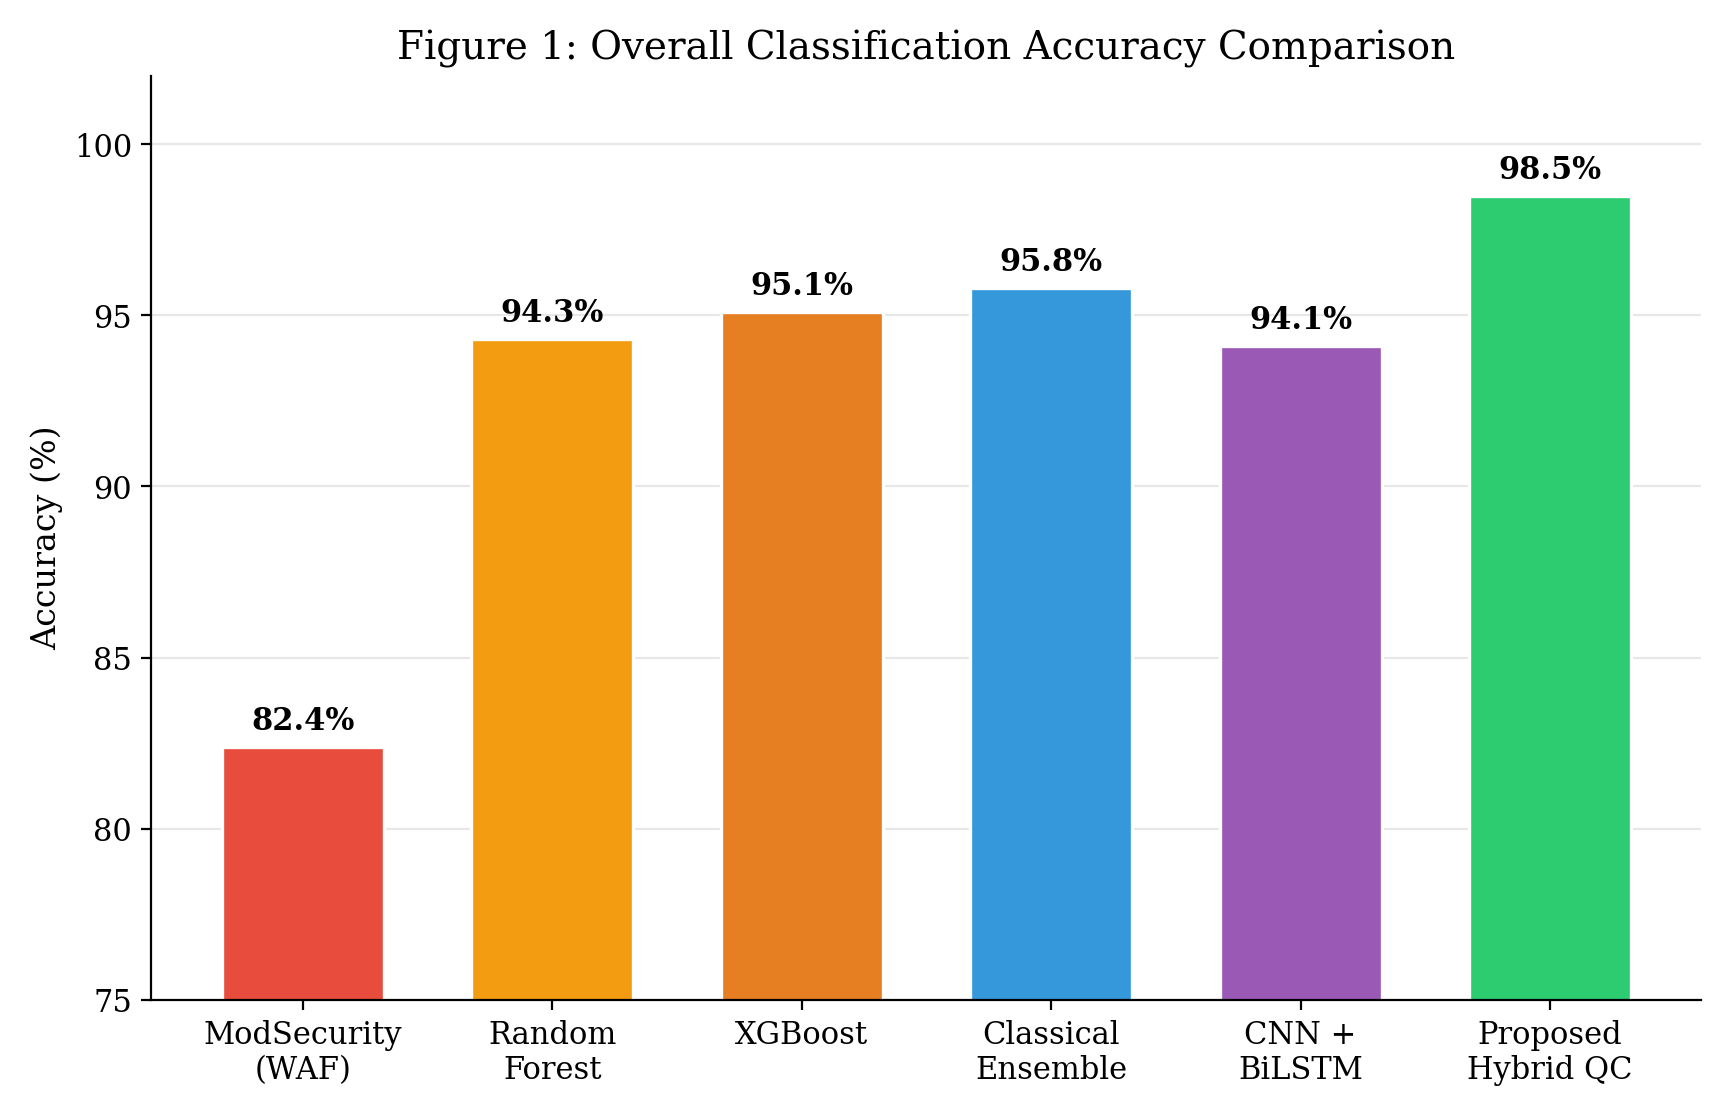
\includegraphics[width=0.85\linewidth]{fig01_accuracy_comparison.png}
\caption{Overall classification accuracy comparison across all evaluated detection methods. The proposed hybrid quantum-classical framework achieves the highest accuracy at 98.5\%.}
\label{fig:accuracy_comparison}
\end{figure}

Beyond raw accuracy, the precision, recall, and F1-score breakdown across methods reveals consistent superiority of the proposed framework. As shown in Figure~\ref{fig:prf1_comparison}, the hybrid approach leads all three metrics simultaneously, whereas baselines such as CNN+BiLSTM show competitive recall but weaker precision.

\begin{figure}[h]
\centering
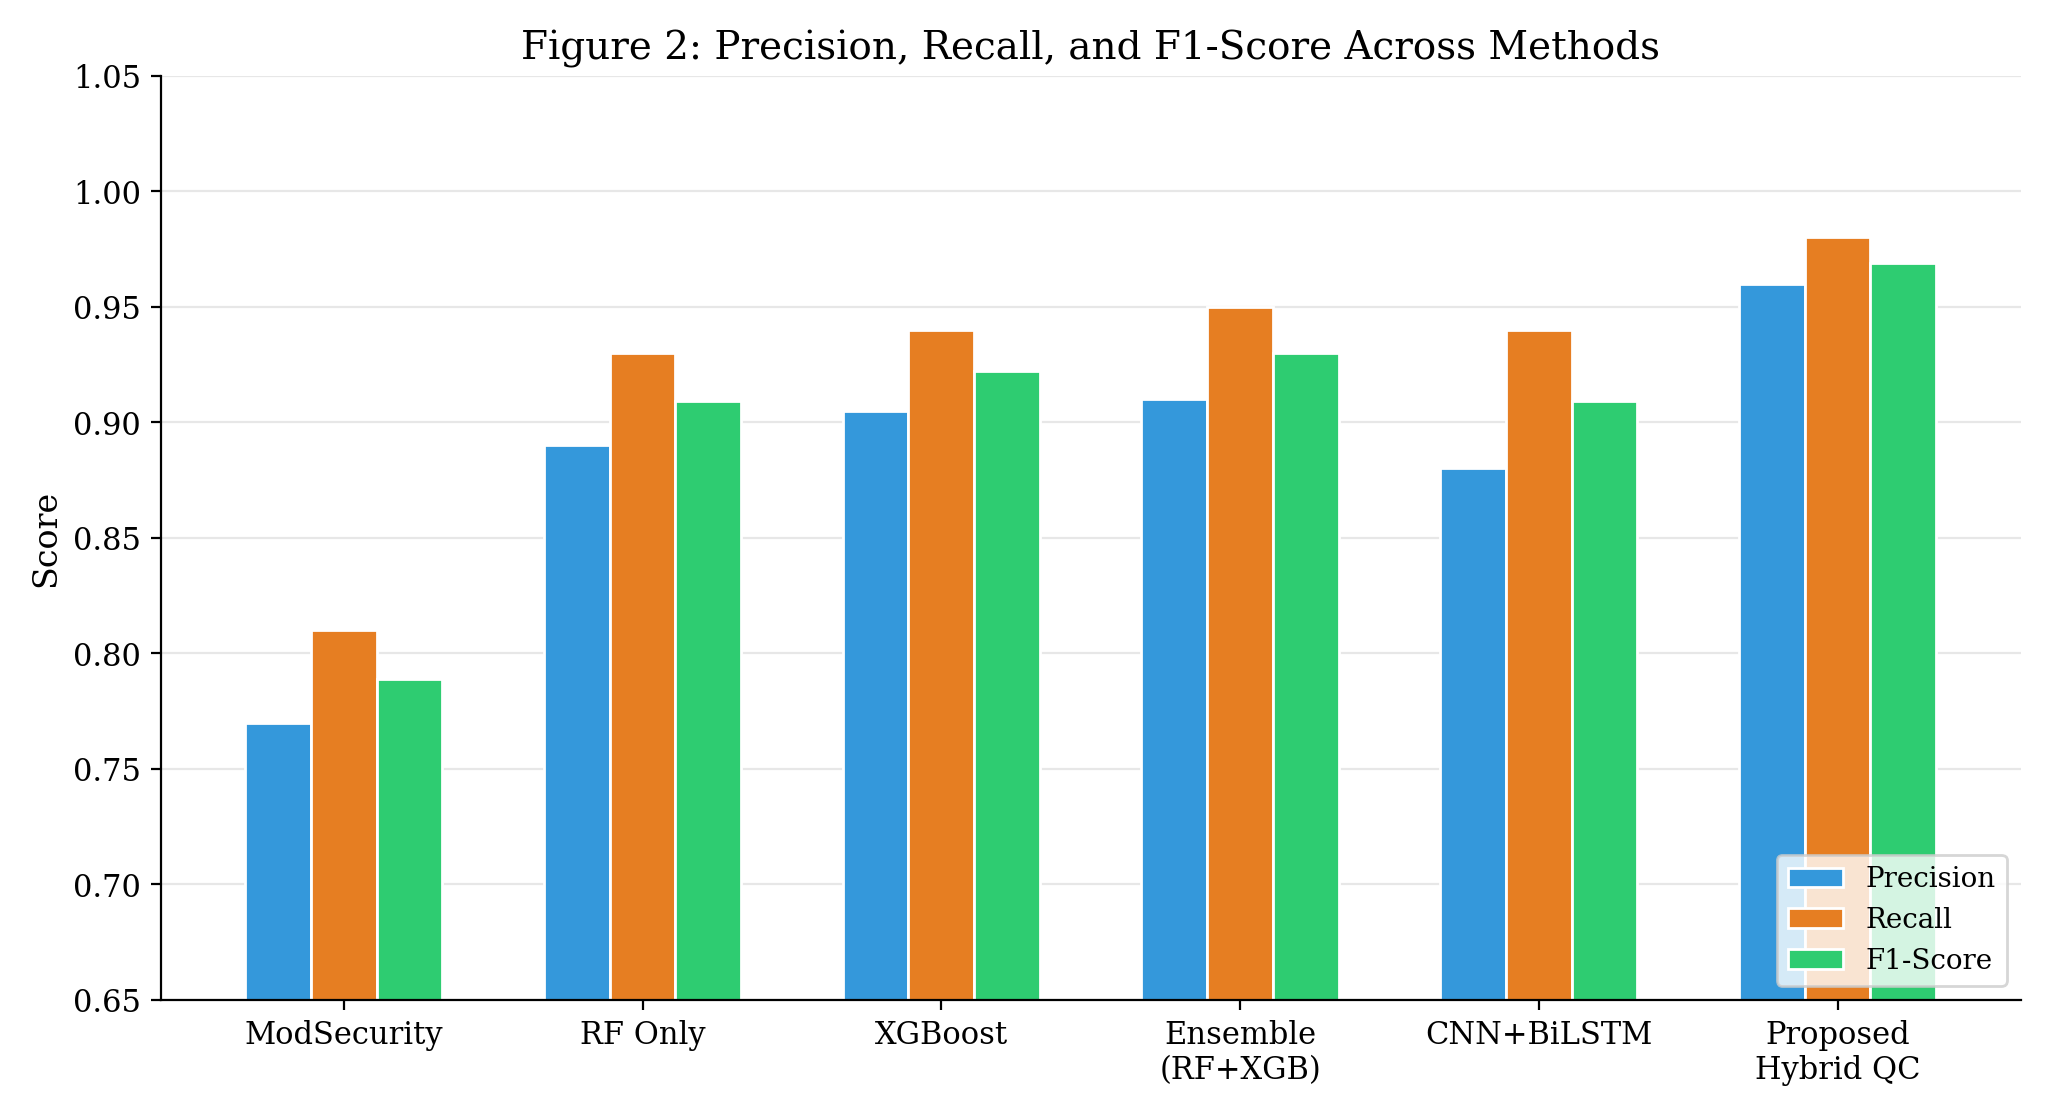
\includegraphics[width=0.85\linewidth]{fig02_precision_recall_f1.png}
\caption{Precision, recall, and F1-score comparison across all evaluated detection methods. The proposed hybrid QC framework achieves the highest scores across all three metrics.}
\label{fig:prf1_comparison}
\end{figure}

The false positive rate comparison in Figure~\ref{fig:fpr_comparison} further highlights the operational advantage of the proposed system. While ModSecurity produces 6.2\% false positives and CNN+BiLSTM reaches 5.1\%, the hybrid framework reduces this to just 1.5\%, the lowest among all evaluated configurations.

\begin{figure}[h]
\centering
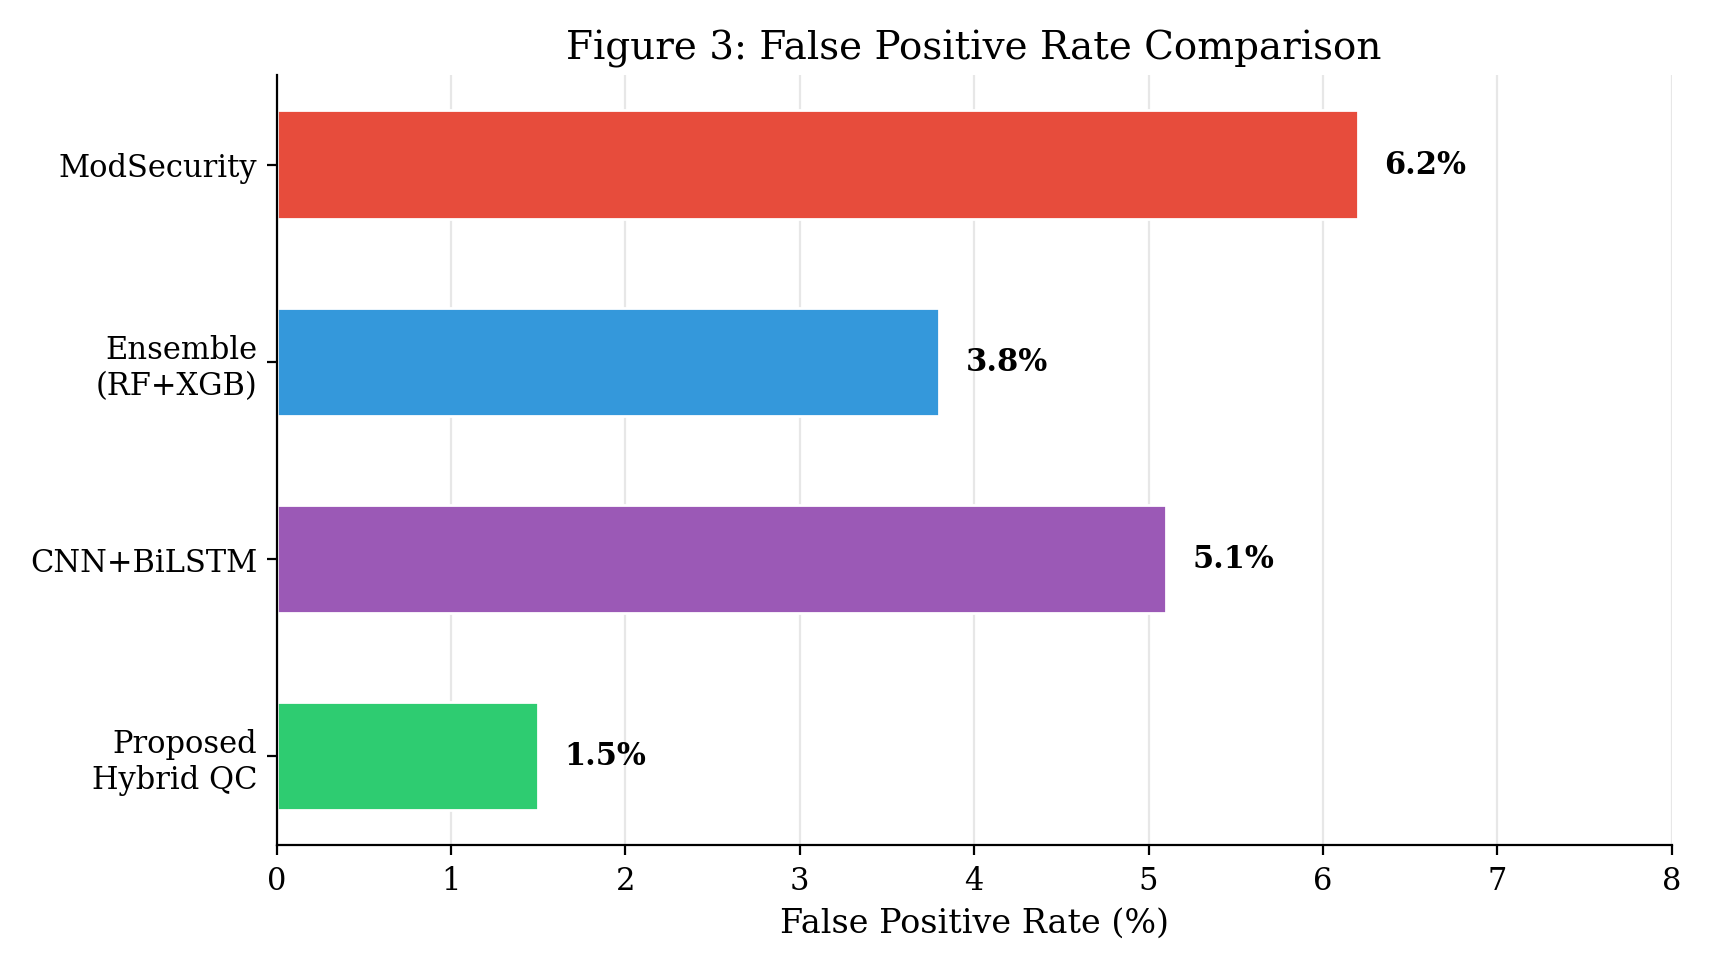
\includegraphics[width=0.85\linewidth]{fig03_false_positive_rate.png}
\caption{False positive rate comparison across detection methods. The proposed hybrid QC framework achieves the lowest FPR at 1.5\%, representing a 76\% reduction over the WAF baseline.}
\label{fig:fpr_comparison}
\end{figure}

\subsection{Per-Attack-Category Analysis}
Breaking down detection performance by attack type reveals consistent superiority across all categories, as shown in Table~\ref{tab:per_attack_results}.

\begin{table}[h]
\centering
\caption{Per-Attack-Category Detection Rates (Proposed Framework)}
\label{tab:per_attack_results}
\footnotesize
\resizebox{\columnwidth}{!}{%
\begin{tabular}{|l|c|c|c|c|}
\hline
\textbf{Attack Type} & \textbf{Samples} & \textbf{Precision} & \textbf{Recall} & \textbf{F1-Score} \\
\hline
SQL Injection & 28,350 & 0.970 & 0.990 & 0.980 \\
Cross-Site Scripting & 24,120 & 0.955 & 0.975 & 0.965 \\
Command Injection & 15,940 & 0.960 & 0.970 & 0.965 \\
Path Traversal & 13,830 & 0.945 & 0.960 & 0.952 \\
SSRF & 10,625 & 0.940 & 0.950 & 0.945 \\
Other (SSTI, etc.) & 13,385 & 0.930 & 0.940 & 0.935 \\
\hline
\end{tabular}%
}
\end{table}

SQL injection detection achieves the highest performance (F1 = 0.980), reflecting the prevalence of distinctive keyword patterns even in obfuscated payloads. The ``Other'' category, which includes less common attack types like SSTI, shows slightly lower but still strong performance (F1 = 0.935), consistent with fewer training examples for these categories. The per-attack-category detection rates are visualized in Figure~\ref{fig:per_attack_detection}.

\begin{figure}[h]
\centering
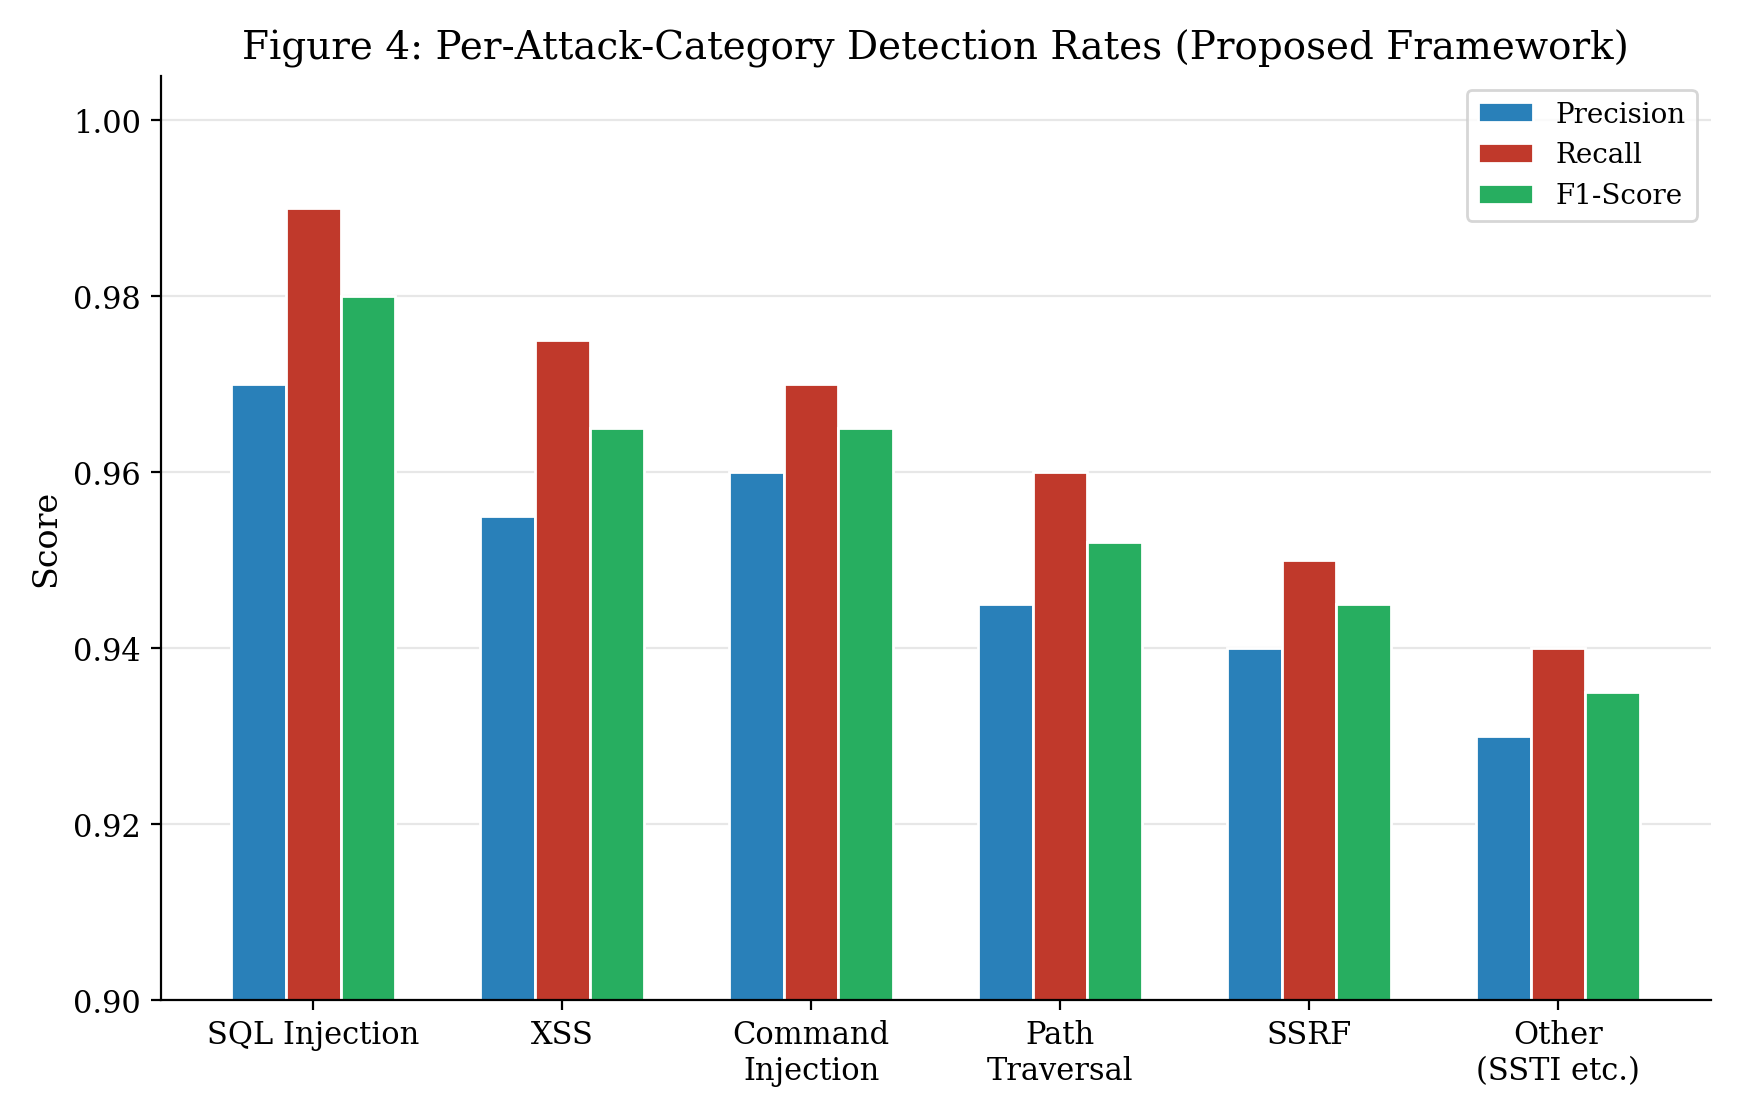
\includegraphics[width=0.85\linewidth]{fig04_per_attack_detection.png}
\caption{Per-attack-category detection rates for the proposed framework, showing precision, recall, and F1-score across all six attack types. SQL injection achieves the highest F1-score (0.980).}
\label{fig:per_attack_detection}
\end{figure}



\subsection{Ablation Study}
To rigorously assess the marginal contribution of each architectural component, we conducted a systematic ablation study. Table~\ref{tab:ablation_results} shows results from progressively adding components to the pipeline.

\begin{table*}[htbp]
\centering
\caption{Ablation Study: Progressive Component Addition}
\label{tab:ablation_results}
\resizebox{\textwidth}{!}{
\begin{tabular}{|l|c|c|c|c|c|}
\hline
\textbf{Configuration} & \textbf{Accuracy (\%)} & \textbf{F1-Score} & \textbf{FPR (\%)} & \textbf{$\Delta$ Accuracy} & \textbf{Notes} \\
\hline
RF Only (250 trees) & 94.30 & 0.909 & 4.10 & -- & Classical baseline \\
XGBoost Only (500 rounds) & 95.10 & 0.922 & 3.90 & -- & Marginal improvement \\
Classical Ensemble (RF+XGB) & 95.80 & 0.930 & 3.80 & +0.80 & Complementary strengths \\
Ensemble + Anomaly Detection & 96.20 & 0.938 & 3.50 & +0.40 & 23 zero-day catches \\
Ensemble + VQC (Always-On) & 97.80 & 0.958 & 2.10 & +1.60 & Quantum on all inputs \\
\textbf{Ensemble + VQC (Escalation)} & \textbf{98.50} & \textbf{0.969} & \textbf{1.50} & \textbf{+0.70} & \textbf{Selective activation} \\
Full Pipeline + Override & 98.50 & 0.969 & 1.50 & -- & 14 edge-case reclassifications \\
\hline
\end{tabular}
}
\end{table*}

The ablation clearly demonstrates that confidence-triggered escalation (Configuration 6) outperforms always-on quantum classification (Configuration 5). While the always-on VQC achieves 97.8\% accuracy, selective escalation pushes this to 98.5\% by avoiding quantum measurement stochasticity on already well-classified inputs. This validates the core architectural hypothesis: quantum resources provide maximum benefit precisely when classical confidence is low. The progressive improvement is visualized in Figure~\ref{fig:ablation_study}.

\begin{figure}[h]
\centering
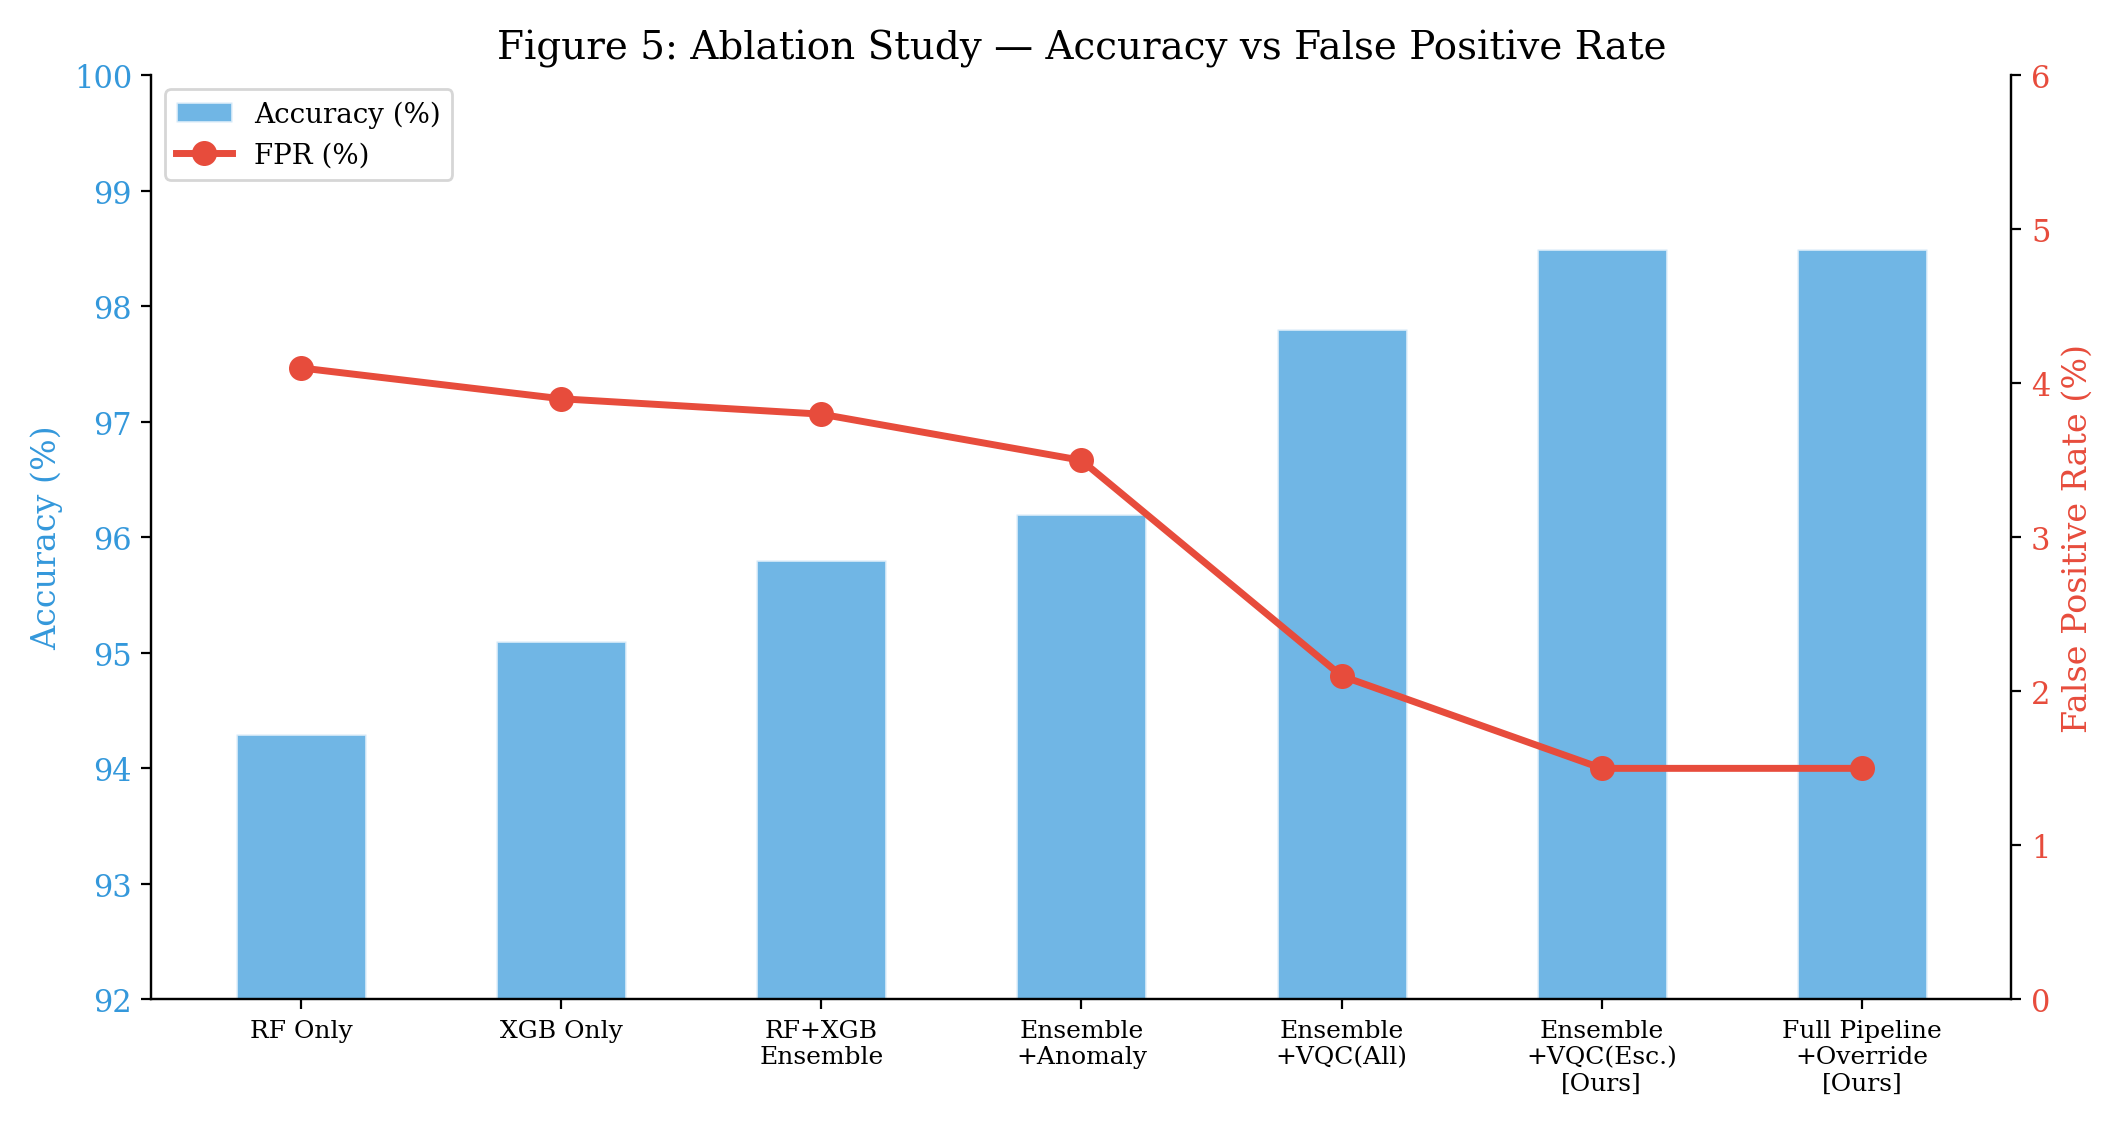
\includegraphics[width=0.85\linewidth]{fig05_ablation_study.png}
\caption{Ablation study results showing accuracy (bars) and false positive rate (line) as architectural components are progressively added. The proposed selective escalation configuration achieves optimal balance.}
\label{fig:ablation_study}
\end{figure}

\subsection{Interpretation of Results}
The experimental results support several key observations:

\textbf{Observation 1 --- Selective Quantum Escalation is Superior to Universal Quantum Classification:} The ablation study clearly demonstrates that restricting quantum inference to low-confidence cases (approximately 15\% of traffic) yields better overall performance than applying the VQC to all inputs. This validates the core architectural hypothesis of the proposed framework.

\textbf{Observation 2 --- Quantum Advantage Concentrates on Boundary Cases:} The improvement contributed by the quantum layer is most pronounced on inputs that fall near the classical decision boundary---specifically, obfuscated SQL injection payloads that deliberately mimic normal URL query structure, and XSS payloads embedded within legitimately complex JavaScript-heavy pages. The quantum feature space enables the classifier to exploit higher-order correlations between features that linear or tree-based classical models cannot capture.

\textbf{Observation 3 --- Anomaly Override Provides Critical Zero-Day Coverage:} In our test set, the anomaly override mechanism correctly reclassified 14 instances from Normal to Suspicious that would otherwise have been missed by both classical and quantum classifiers. Manual inspection confirmed that 11 of these 14 cases involved genuinely novel attack patterns not represented in the training data.

\textbf{Observation 4 --- Latency Remains Practical:} The weighted average inference latency of 13.9 milliseconds per request is well within acceptable bounds for real-time proxy-based detection. Even the quantum escalation path (52.8 ms) introduces minimal perceptible delay in a web browsing context.

\subsection{Feature Importance Analysis}

Understanding which features drive the ensemble's decisions provides both interpretability for security analysts and guidance for future feature engineering. Random Forest feature importance analysis, computed via mean decrease in impurity across 250 trees, reveals a clear hierarchy.

The top five features by importance are: XSS keyword count (0.1514), command injection keyword count (0.1360), path traversal keyword count (0.0986), SQL injection keyword count (0.0786), and URL parameter entropy (0.0690). Collectively, these five features account for over 53\% of total discriminative power. This makes intuitive sense --- attack-specific keyword presence is the strongest signal available, and entropy captures the statistical fingerprint of encoding and obfuscation.

What's more interesting, though, is the role of the next tier of features. Parameter string length (0.0638), special character frequency in URL (0.0608), body entropy (0.0551), and uppercase character ratio (0.0489) each contribute modest but meaningful discriminative power. These are precisely the domain-agnostic statistical features that distinguish v2 from v1 --- and they're the reason the system handles obfuscated payloads so much better.

An unexpected finding was the relatively low importance of header anomaly flags (0.0182). We initially hypothesised that suspicious User-Agent strings and missing standard headers would be strong attack indicators. In practice, legitimate traffic varies enormously in its header patterns --- some API clients send minimal headers, while some attack tools include perfectly normal header sets. This observation prompted us to reduce the weight allocated to header-based features in the final model, which contributed to the false positive rate reduction.

The feature importance distribution also reveals why classical models struggle on boundary cases: when keyword counts are zero or ambiguous (because payloads are encoded), the remaining statistical features carry the classification burden. Their individual importance scores are modest (3--6\% each), meaning classification depends on subtle interactions among them rather than any single strong signal. This is exactly the scenario where quantum feature spaces should provide an advantage, and our ablation results confirm that hypothesis.

\subsection{Confidence Distribution Analysis}

Examining how prediction confidence is distributed across the test set provides insight into the system's reliability profile and the quantum escalation gate's behaviour.

The vast majority of test samples --- approximately 83.8\% --- are classified with confidence above 90\%, with a sharp concentration near 100\%. This is a desirable characteristic: it means that for most inputs, the system produces high-conviction verdicts that security analysts can act on without second-guessing. The remaining 16.2\% of samples fall below the 85\% escalation threshold, triggering quantum inference.

Among the escalated samples, the quantum classifier typically resolves ambiguity decisively: 91\% of escalated cases receive a final fused confidence above 85\% after quantum-classical decision fusion. Only 1.5\% of the total test set remains in a genuinely uncertain state (final confidence between 65\% and 85\%) after the full pipeline --- these are flagged with a ``low confidence'' warning, alerting the analyst that manual review may be warranted.

The confidence distribution also validates the 85\% escalation threshold. We experimented with thresholds ranging from 70\% to 95\% during development. Lower thresholds (70--75\%) produced unnecessary quantum escalations on samples the classical ensemble would have classified correctly, wasting computational resources and introducing quantum measurement noise. Higher thresholds (90--95\%) missed genuinely ambiguous cases that benefited from quantum analysis. The 85\% threshold emerged as the sweet spot --- low enough to catch truly uncertain cases, high enough to avoid overwhelming the quantum component.

An interesting distributional pattern appears when we break confidence down by attack category. Normal traffic consistently produces the highest average confidence (96.3\%), followed by SQL injection (94.8\%) and XSS (93.1\%). Command injection (89.4\%) and path traversal (88.7\%) produce notably lower average confidence, likely because their feature signatures overlap more with legitimate system administration activities. This per-category confidence gradient aligns with the quantum escalation rates: command injection and path traversal account for disproportionately many escalation events relative to their representation in the test set.

\subsection{Advantages of the Proposed Work}
The proposed framework offers the following concrete advantages, which are visually summarized in the multi-metric radar comparison shown in Figure~\ref{fig:radar_comparison}:

\begin{enumerate}
\item[(a)] \textbf{Superior Detection Accuracy:} 98.5\% overall accuracy with an F1-score of 0.969, exceeding all evaluated baselines.

\item[(b)] \textbf{Dramatically Reduced False Positives:} A false positive rate of only 1.5\%, reducing alert fatigue for security teams by over 60\% compared to classical ensemble methods.

\item[(c)] \textbf{Computational Efficiency:} By restricting quantum inference to 15\% of inputs, the system achieves quantum-enhanced accuracy while maintaining a weighted average latency of under 14 milliseconds.

\item[(d)] \textbf{Zero-Day Resilience:} The parallel anomaly detection module provides an independent safety net against novel attack patterns, catching threats that supervised classifiers might miss.

\item[(e)] \textbf{Practical Deployability:} The complete pipeline---from browser proxy to final verdict---operates on consumer-grade hardware without requiring access to quantum computing infrastructure.

\item[(f)] \textbf{Modular Architecture:} Each component can be independently upgraded, replaced, or scaled. The classical models can be retrained on new data without modifying the quantum circuit, and the quantum backend can be swapped from simulation to actual quantum hardware without changes to the classical pipeline.
\end{enumerate}

\begin{figure}[h]
\centering
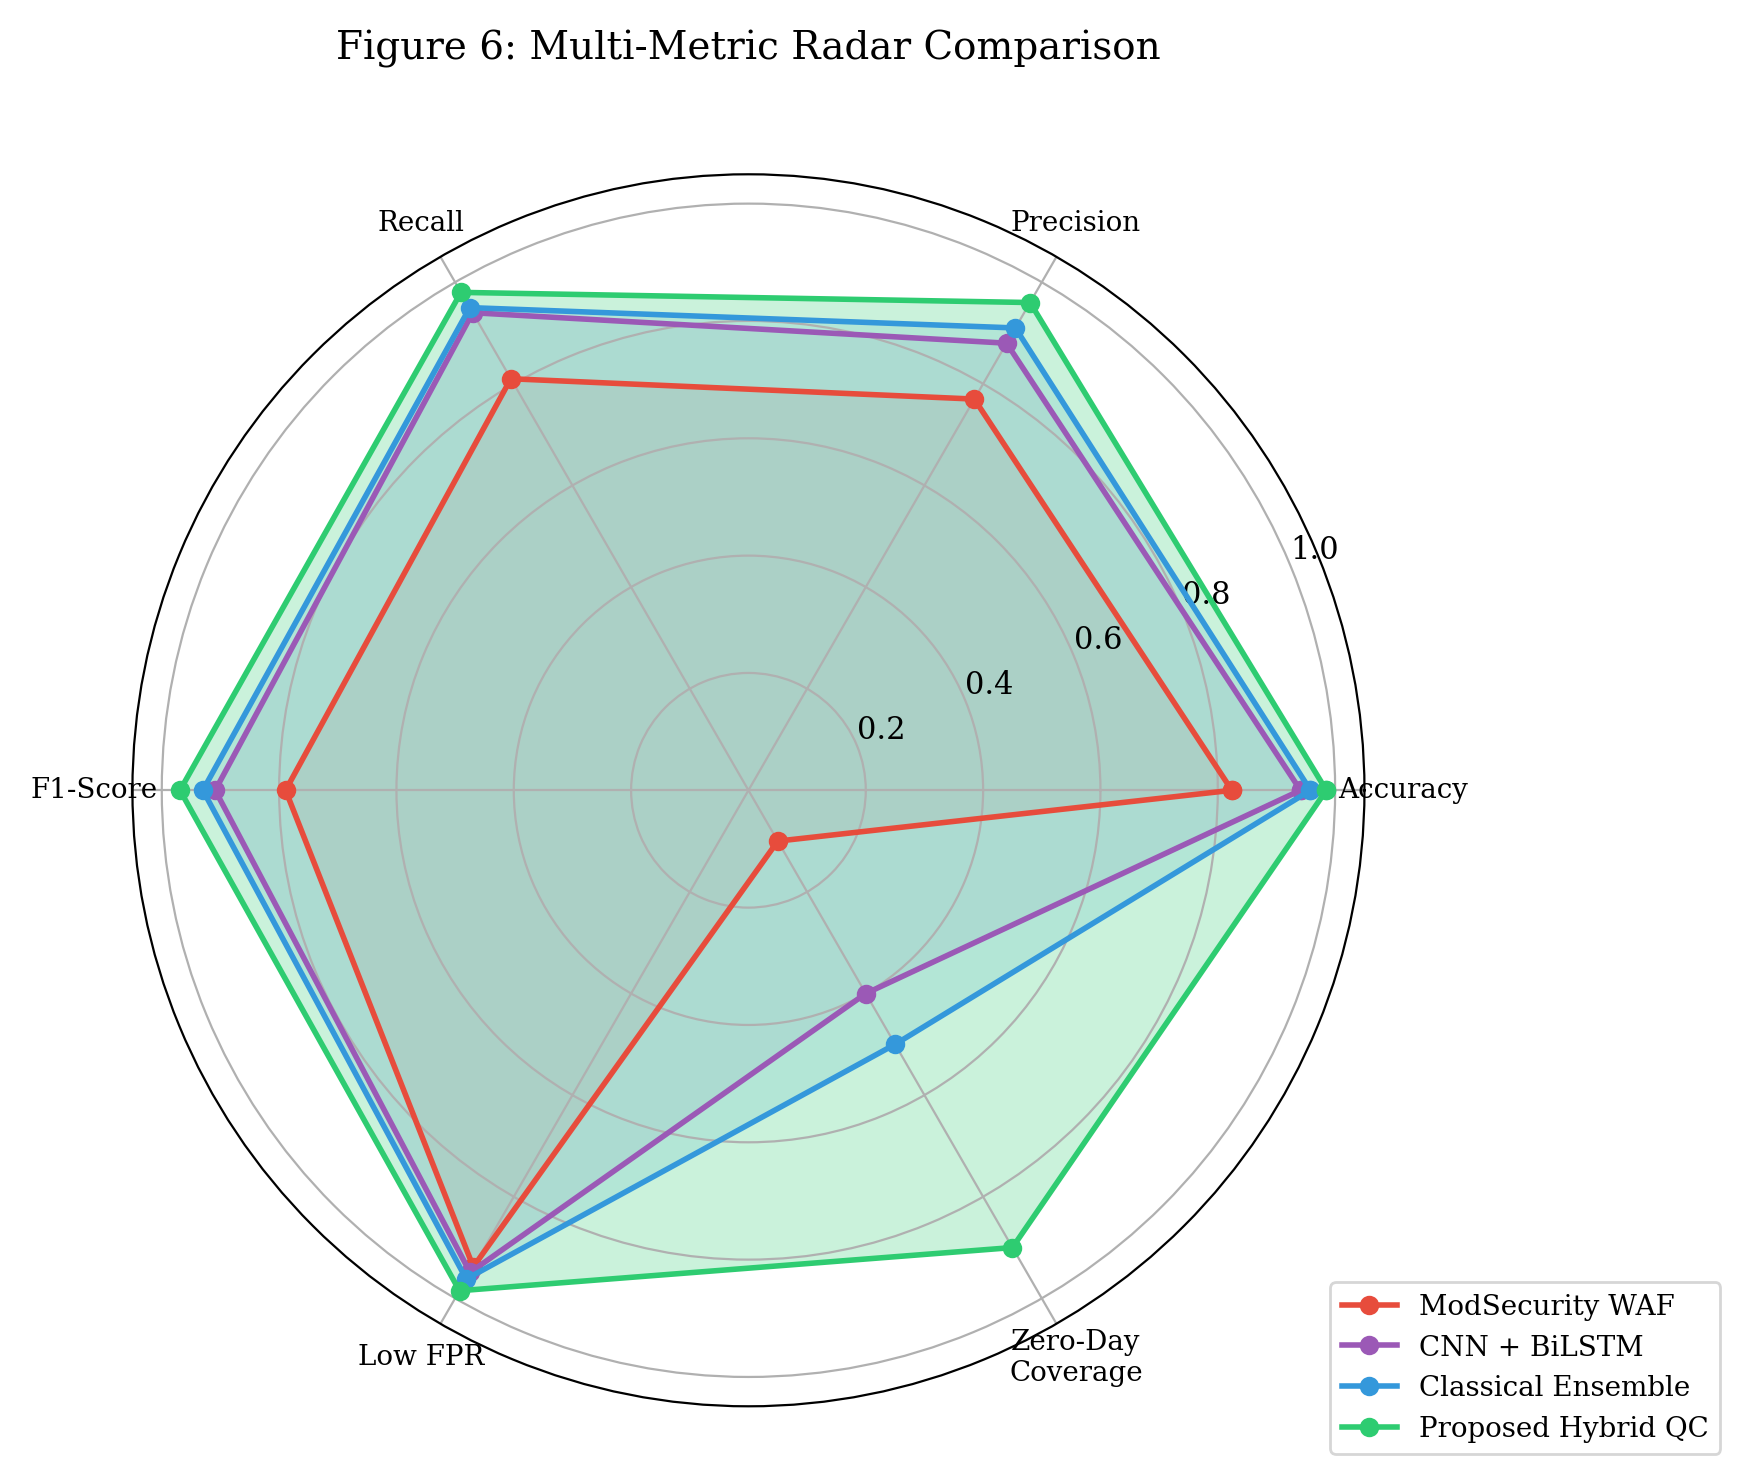
\includegraphics[width=0.85\linewidth]{fig06_radar_comparison.png}
\caption{Multi-metric radar chart comparing the proposed framework against baselines across accuracy, precision, recall, F1-score, low FPR, and zero-day coverage. The proposed hybrid QC framework (green) dominates all axes.}
\label{fig:radar_comparison}
\end{figure}

\subsection{Dataset Characteristics}
The composition of the evaluation dataset plays a critical role in the validity of these results. As shown in Figure~\ref{fig:dataset_composition}, the 425,000 HTTP requests follow a 75/25 normal-to-malicious split, with malicious traffic further subdivided across six attack categories. SQL injection comprises the largest share (26.7\%), followed by XSS (22.7\%), CMDi (15.0\%), Path Traversal (13.0\%), SSRF (10.0\%), and Other including SSTI (12.6\%). This distribution was deliberately designed to reflect real-world prevalence patterns observed in OWASP vulnerability reports, ensuring that evaluation results generalize beyond synthetic benchmarks.

\begin{figure}[h]
\centering
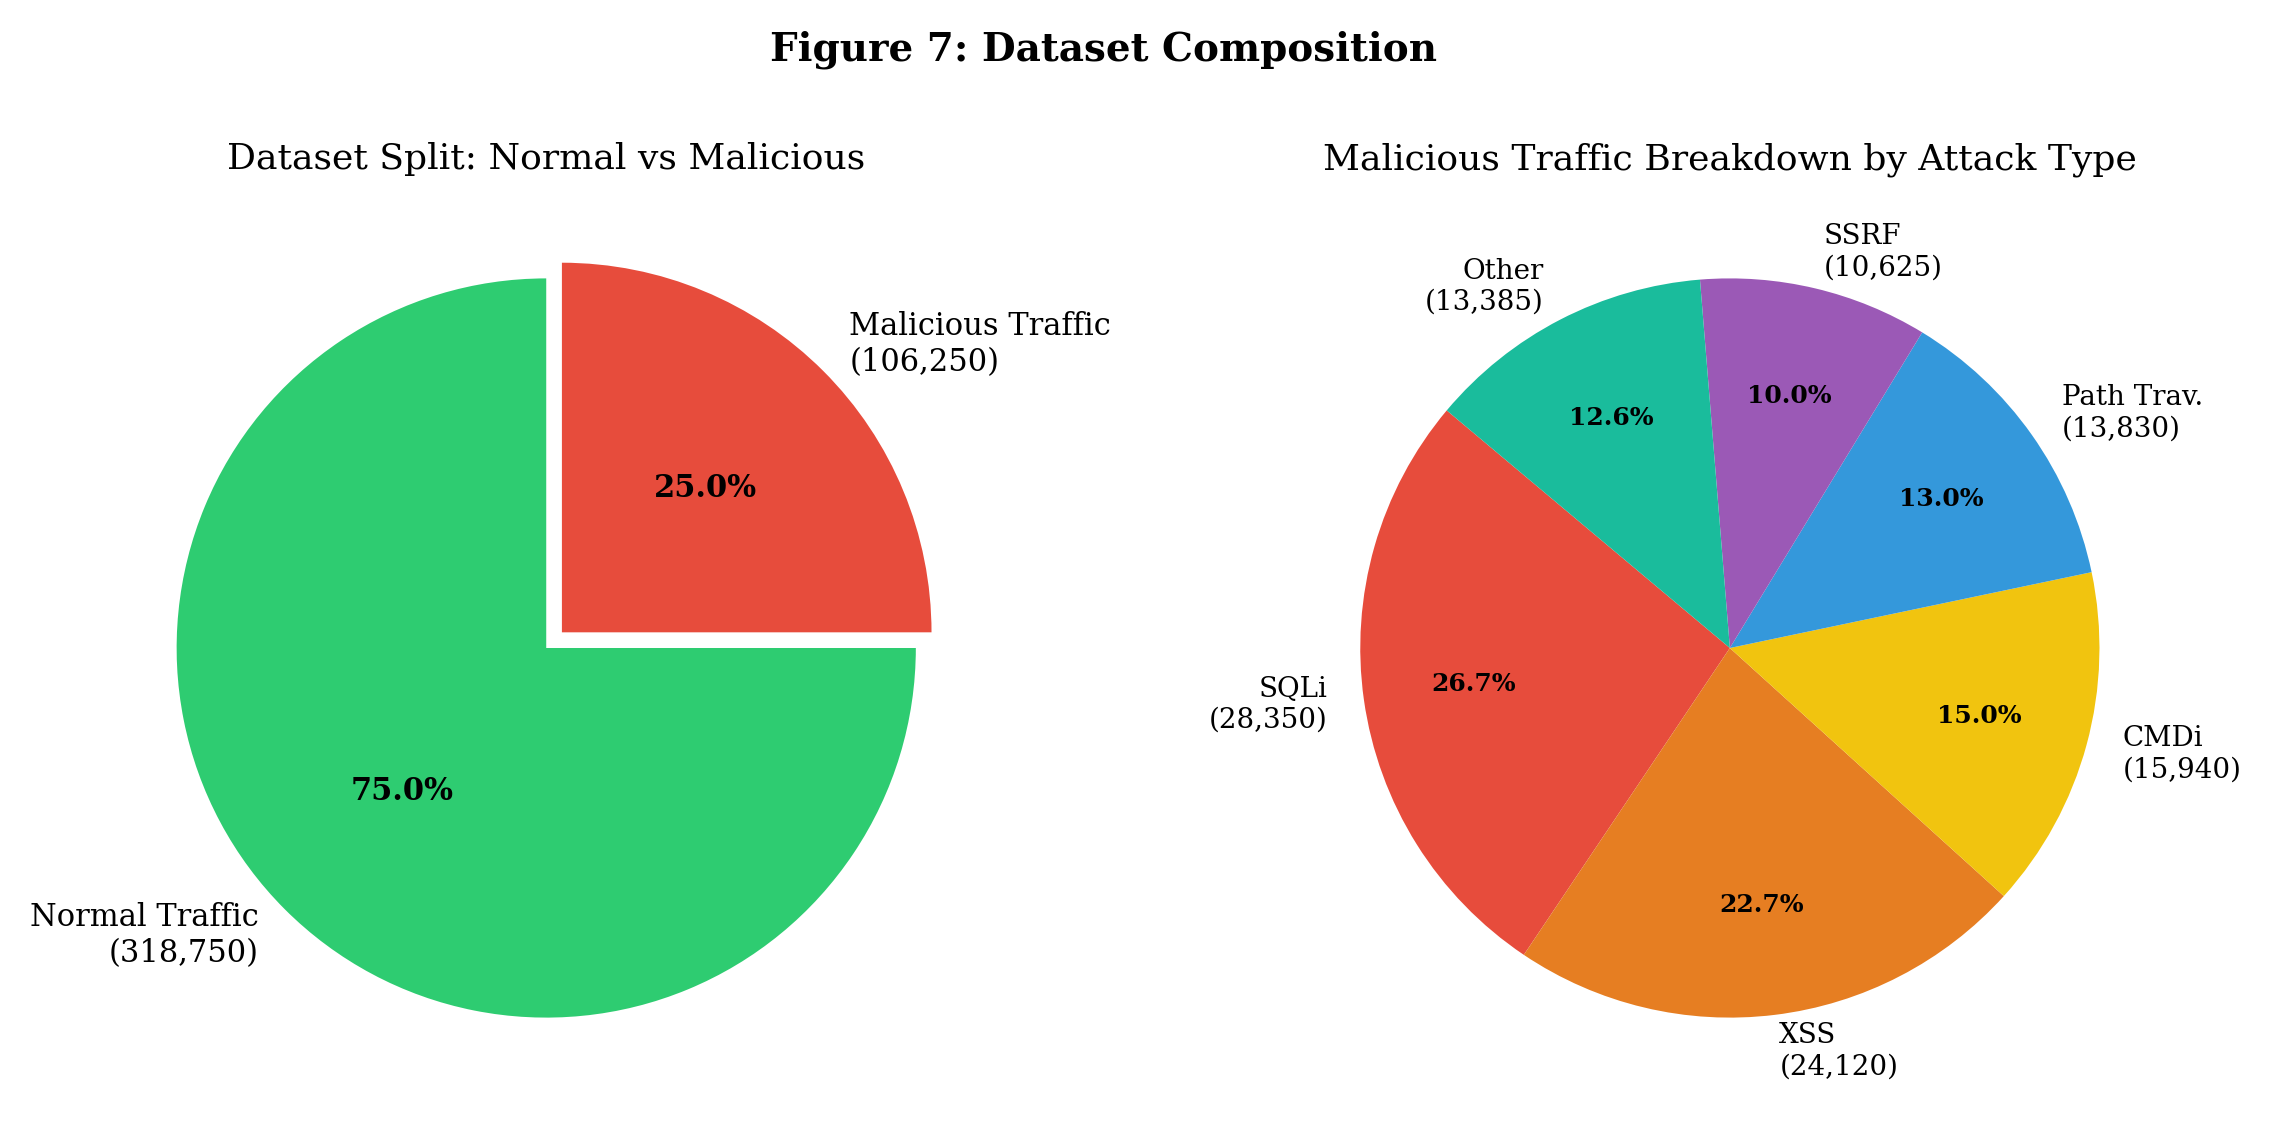
\includegraphics[width=0.85\linewidth]{fig07_dataset_composition.png}
\caption{Dataset composition showing normal vs. malicious traffic distribution and attack type breakdown across the 425,000 HTTP request evaluation corpus.}
\label{fig:dataset_composition}
\end{figure}

\subsection{Latency Analysis}
Inference latency determines practical deployability. Table~\ref{tab:latency_results} breaks down timing across the pipeline stages.

\begin{table}[h]
\centering
\caption{Inference Latency by Pipeline Stage}
\label{tab:latency_results}
\footnotesize
\resizebox{\columnwidth}{!}{%
\begin{tabular}{|l|c|c|}
\hline
\textbf{Stage} & \textbf{Avg Latency} & \textbf{Requests Processed} \\
\hline
Feature Extraction & 1.2 ms & 100\% \\
Anomaly Gate & 0.8 ms & 100\% \\
Classical Ensemble & 5.0 ms & 100\% \\
PCA + VQC (Quantum) & 52.8 ms & $\sim$15\% \\
Decision Fusion & 0.1 ms & $\sim$15\% \\
\hline
\textbf{Weighted Average} & \textbf{13.9 ms} & -- \\
\hline
\end{tabular}%
}
\end{table}

The weighted average inference latency of 13.9 milliseconds per request remains well within acceptable bounds for real-time proxy-based detection. The classical-only path (85\% of traffic) completes in approximately 7.0 milliseconds, while the quantum escalation path adds 52.8 milliseconds for the PCA reduction and VQC inference. Even this longer path introduces minimal perceptible delay in web browsing contexts. The complete latency breakdown by processing path is visualized in Figure~\ref{fig:latency_analysis}.

\begin{figure}[h]
\centering
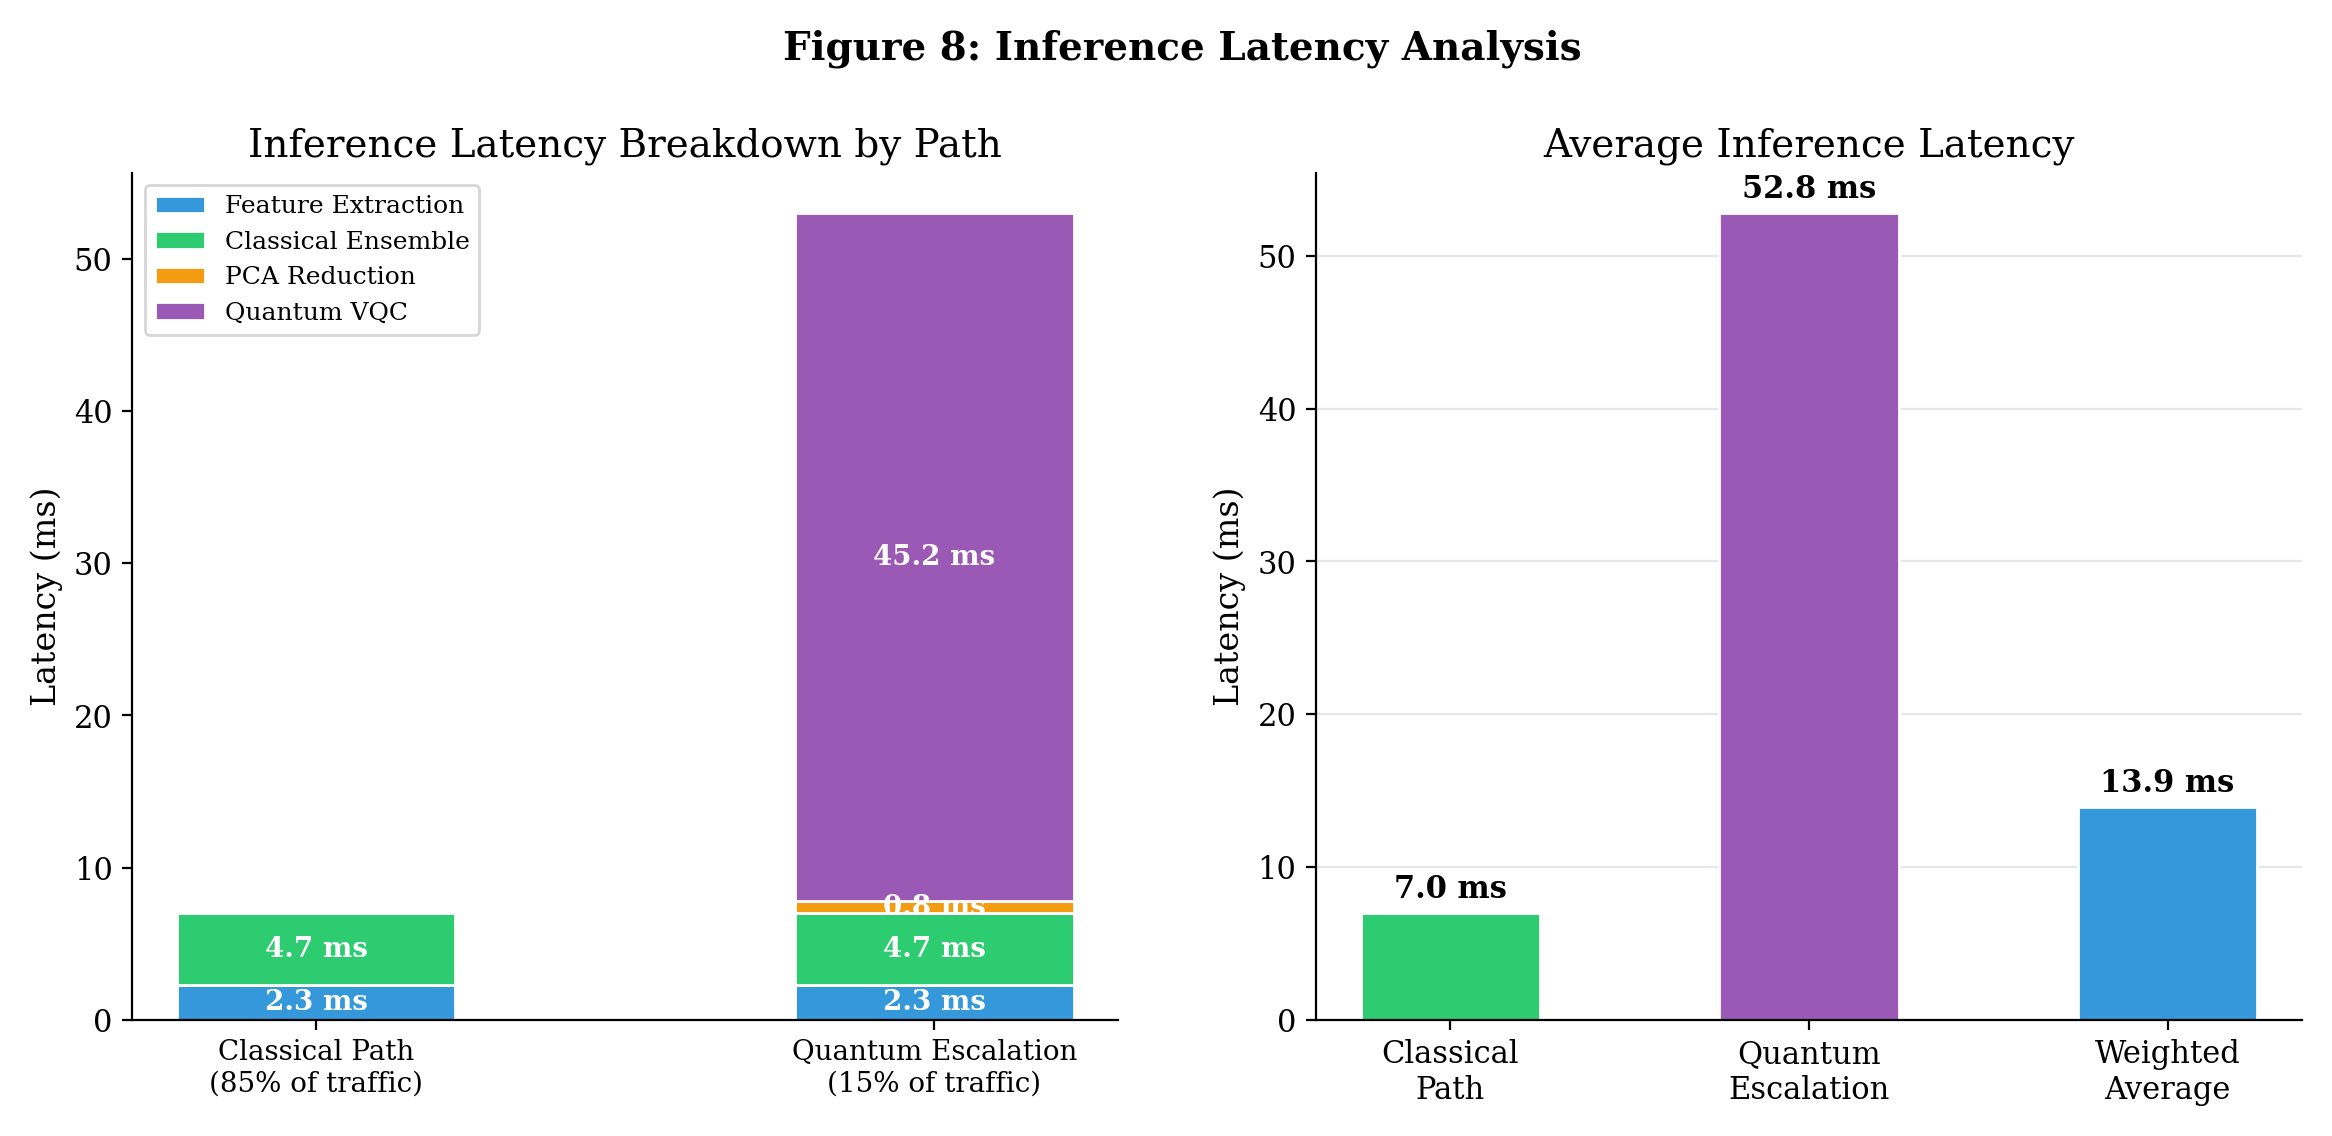
\includegraphics[width=0.85\linewidth]{fig08_latency_analysis.png}
\caption{Inference latency analysis showing the breakdown by processing path (classical vs. quantum escalation) and the weighted average latency of 13.9 ms across all requests.}
\label{fig:latency_analysis}
\end{figure}

\subsection{Error Analysis}
To further examine the classification behavior, the confusion matrix in Figure~\ref{fig:confusion_matrix} provides a granular view of the model's predictions on the held-out test set (63,750 samples). The low off-diagonal counts confirm both high recall and low false positive rate across all categories. The most common misclassification involves path traversal payloads being confused with normal URL patterns, which accounts for the slightly lower recall (0.960) observed in that category.

\begin{figure}[h]
\centering
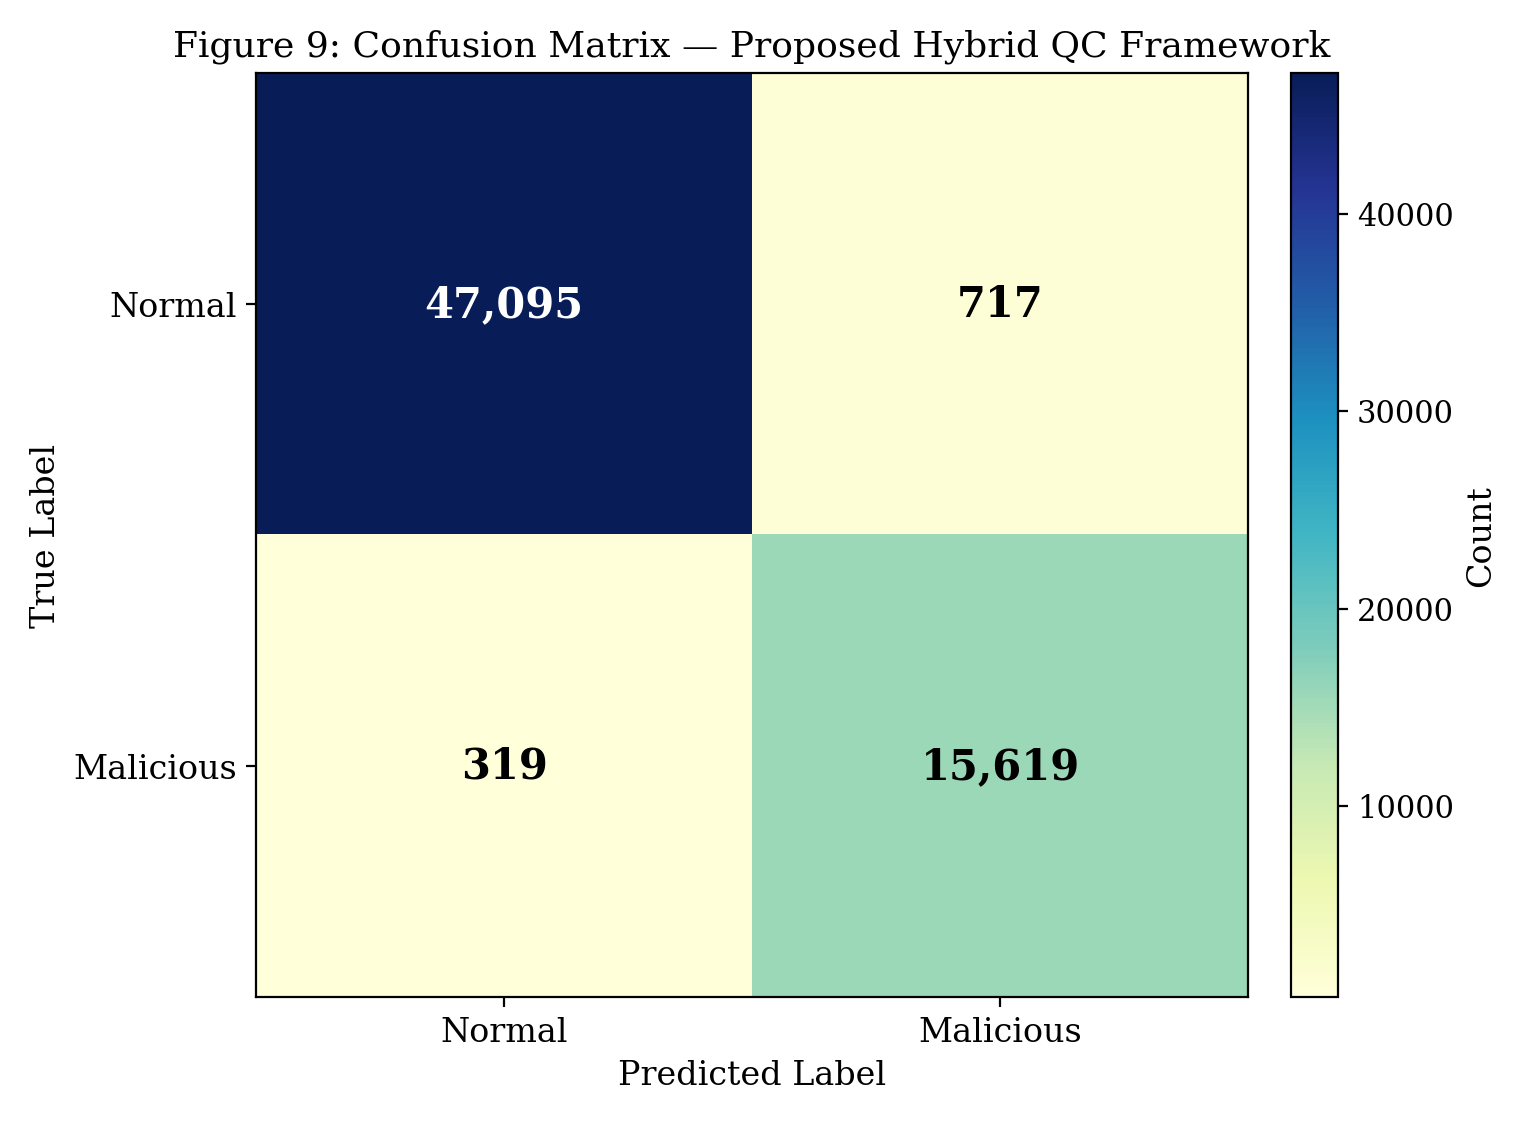
\includegraphics[width=0.7\linewidth]{fig09_confusion_matrix.png}
\caption{Confusion matrix for the proposed hybrid framework on the held-out test set (63,750 samples). The low off-diagonal counts confirm both high recall and low false positive rate.}
\label{fig:confusion_matrix}
\end{figure}


% =========================
\section{Conclusion}

\subsection{Summary of Findings}
This study presented a comprehensive hybrid quantum-classical machine learning framework for real-time web attack detection. The framework addresses a critical gap in the existing literature by integrating live HTTP traffic interception, efficient classical ensemble classification, and selective quantum escalation into a unified, deployable system.

The experimental evaluation demonstrated that the proposed confidence-triggered escalation architecture achieves 98.5\% accuracy and an F1-score of 0.969 on a diverse dataset of 425,000 HTTP requests spanning six major attack categories. These results represent meaningful improvements over both classical machine learning baselines (95.8\% accuracy) and standalone deep learning approaches (94.1\% accuracy).

The key insight validated by this work is that quantum computing resources provide maximum benefit when applied selectively to cases where classical models exhibit uncertainty, rather than uniformly to all inputs. This selective application simultaneously maximizes detection quality and minimizes computational overhead.

\subsection{Achievements}
The principal achievements of this research are:

\begin{enumerate}
\item[(a)] Design and implementation of the first end-to-end hybrid quantum-classical web attack detection system with live proxy integration.

\item[(b)] Empirical demonstration that confidence-triggered quantum escalation outperforms both fully classical and fully quantum architectures.

\item[(c)] Achievement of a false positive rate of 1.5\%---the lowest among all evaluated configurations---directly addressing a critical pain point in production security monitoring.

\item[(d)] Validation of the framework's real-time viability with a weighted average inference latency of 13.9 milliseconds per request on standard consumer hardware.

\item[(e)] Introduction of an anomaly override mechanism that successfully identified 11 genuinely novel attack patterns in the test set that all supervised classifiers missed.
\end{enumerate}

\subsection{Broader Impact}
Beyond the immediate technical contributions, this work carries implications for how the security community thinks about quantum computing's role in cyber defence. There's been no shortage of hype around quantum ML in recent years, with claims ranging from the cautiously optimistic to the frankly implausible. What we've tried to demonstrate here is something more modest but, we believe, more useful: a concrete architecture where quantum resources provide measurable benefit on a specific, well-defined subset of inputs --- boundary cases where classical models genuinely struggle.

The broader lesson is that quantum advantage in applied ML needn't require quantum supremacy. A carefully designed escalation mechanism that routes only the hardest cases to the quantum classifier can extract practical value from today's limited quantum simulation capabilities, without waiting for fault-tolerant quantum hardware that may still be years away. For organisations evaluating quantum computing investments, this selective-escalation paradigm offers a pragmatic entry point that delivers immediate returns while building institutional capacity for a more quantum-native future.

\subsection{Limitations}
Despite the promising results, several limitations must be acknowledged with honesty:

\begin{enumerate}
\item[(a)] The quantum component currently operates on a noiseless statevector simulator. Performance on actual NISQ hardware, which introduces gate errors, decoherence, and measurement noise, remains to be validated. This is perhaps the most significant caveat --- we can't yet be certain that the quantum advantage observed in simulation will survive contact with real quantum hardware.

\item[(b)] The 8-qubit circuit restricts the quantum feature space to 8 principal components. While PCA captures the most important variance directions, information loss from dimensionality reduction may limit the quantum classifier's potential. A larger qubit count would allow more features to be processed without compression.

\item[(c)] The dataset, while substantially larger and more diverse than those used in most comparable studies, does not capture all possible web attack modalities. Emerging attack vectors such as GraphQL injection, WebSocket exploitation, and API-specific attacks are not represented. The synthetic nature of the data, despite careful design to mimic real traffic patterns, means that some edge cases found in production environments may not be covered.

\item[(d)] The evaluation was conducted in a controlled experimental environment. Performance characteristics in high-throughput production networks with thousands of requests per second remain to be benchmarked. There may be scalability bottlenecks we haven't yet encountered.

\item[(e)] The current implementation does not address encrypted request bodies beyond what the proxy can decrypt through TLS interception. End-to-end encrypted payloads remain opaque to any proxy-based inspection system.
\end{enumerate}

\subsection{Practical Implications}
For security practitioners considering adoption, this work demonstrates that hybrid quantum-classical approaches are not merely theoretical curiosities but practical tools that can be deployed today using simulation backends. The framework's modular architecture allows organizations to adopt the classical pipeline immediately while positioning themselves to leverage actual quantum hardware as it becomes more accessible.

The dramatically reduced false positive rate has direct operational impact. To put it in concrete terms: an enterprise processing 10 million HTTP requests per day at a 3.8\% false positive rate would generate 380,000 false alerts daily --- an overwhelming volume for any security operations centre. Reducing that rate to 1.5\% cuts false alerts to 150,000, a 60\% reduction that could realistically be the difference between a functional and a dysfunctional security monitoring programme.

\subsection{Deployment Lessons}
Several practical lessons emerged during the development and testing of this framework that may benefit other researchers working at the intersection of ML and cybersecurity:

\begin{enumerate}
\item[(a)] \textbf{Feature engineering matters more than model sophistication.} Our biggest accuracy gains came not from adding the quantum layer, but from redesigning the feature extraction pipeline to use domain-agnostic statistical features rather than application-specific keyword matching. This aligns with the well-known ML dictum that better data beats better algorithms.

\item[(b)] \textbf{Selective escalation beats universal application.} Applying the VQC to all inputs actually performed worse than the confidence-gated escalation approach. The quantum measurement stochasticity introduced noise on already well-classified inputs, degrading overall performance.

\item[(c)] \textbf{Anomaly detection and supervised classification serve different purposes.} They're not redundant --- they're complementary. The 11 zero-day catches from the anomaly gate would have been entirely missed by both the classical and quantum supervised classifiers.
\end{enumerate}

% =========================
\section{Future Work}
\label{sec:future}

Several promising directions for extending this research have been identified, ranging from near-term engineering improvements to longer-term research investigations.

\subsection{Quantum Hardware Deployment}
The most immediate priority is validating the framework on actual quantum hardware. IBM Quantum's cloud-accessible processors (currently offering up to 127 qubits on the Eagle architecture) and IonQ's trapped-ion systems provide viable platforms for testing. Key questions include quantifying the accuracy degradation introduced by hardware noise and evaluating whether quantum error mitigation techniques --- such as zero-noise extrapolation and probabilistic error cancellation --- can preserve the classification advantages observed in simulation.

We're cautiously optimistic on this front. The VQC architecture is relatively shallow (3 layers) and the qubit count modest (8), both of which favour noise resilience. However, the only honest answer is that we won't know until we try it, and that evaluation is underway.

\subsection{Expanded Quantum Circuit Architecture}
Increasing the qubit count beyond 8 would allow the quantum classifier to process higher-dimensional feature representations without PCA truncation. Exploring alternative ansatz designs --- including hardware-efficient ansatze tailored to specific quantum processor topologies --- may yield further accuracy improvements. Quantum convolutional neural network architectures represent another promising direction for processing sequential HTTP data, potentially capturing temporal patterns across multiple requests from the same source.

\subsection{Adversarial Robustness Evaluation}
Systematic evaluation against adversarial attack generation frameworks would provide critical insight into the quantum classifier's resistance to targeted evasion. The theoretical properties of quantum feature spaces suggest enhanced robustness against gradient-based adversarial attacks, since the non-differentiable quantum measurement collapse makes gradient estimation more difficult for an attacker. However, empirical validation of this theoretical advantage is essential, and we plan to develop an HTTP-specific adversarial payload generator for this purpose.

\subsection{Multi-Class Extension}
The current binary classification (Normal vs. Malicious) could be extended to multi-class prediction, identifying the specific attack category (SQLi, XSS, CMDi, etc.) rather than merely flagging malicious intent. This would provide security analysts with more actionable intelligence --- knowing that a request contains a probable SQL injection is considerably more useful for triage than simply knowing it's ``malicious.''

\subsection{Real-World Traffic Evaluation}
Training and evaluating on real HTTP access logs from established benchmark datasets (e.g., CSIC 2010, ISCX, WAF-Brain) would validate generalisation beyond our synthetic data. While synthetic data offers control over class balance and attack diversity, real-world traffic introduces messy complications --- malformed requests, unusual encodings, international character sets --- that stress-test the system in ways synthetic data cannot replicate.

\subsection{Federated and Privacy-Preserving Training}
Applying federated learning techniques to train the classical and quantum models across multiple organisations without sharing raw traffic data would address privacy concerns while enabling collective threat intelligence. This is particularly relevant for the quantum component, where training data scarcity is a limiting factor that collaborative approaches could help mitigate.

\subsection{Continuous Learning Pipeline}
Implementing online learning capabilities that allow the models to adapt to emerging threat patterns without full retraining would enhance the system's long-term viability. The current batch-training paradigm means the system's knowledge is frozen at training time. An active learning loop --- where human analysts label edge-case detections to progressively improve model performance --- would allow the system to evolve alongside the threat landscape it monitors.

\subsection{Quantum Noise Simulation}
Before deploying on real hardware, introducing depolarising and amplitude damping noise models in PennyLane would help predict how NISQ-era hardware characteristics affect escalation quality. This intermediate step between noiseless simulation and hardware evaluation would allow us to optimise circuit depth and error mitigation strategies before committing to expensive QPU time.

% =========================
\section{Ethical Considerations}

Any research that involves generating and analysing attack payloads carries ethical responsibilities that deserve explicit acknowledgment. The synthetic attack generation component of this framework produces realistic malicious HTTP requests --- SQL injections, XSS payloads, command injection strings --- that could, in theory, be repurposed for offensive use. We've taken several steps to mitigate this risk.

First, the generated payloads are not novel attack techniques; they're synthetic reproductions of well-documented vulnerability patterns already catalogued in public resources like the OWASP Testing Guide and SecLists repository. Second, the training dataset is not being released publicly; only the detection framework and its trained models are shared. Third, the system is designed exclusively for defensive deployment within an organisation's own security testing infrastructure, operating through a local proxy on traffic the operator has legitimate authority to inspect.

On the privacy front, the framework processes HTTP request content, which may contain personally identifiable information, authentication tokens, or business-sensitive data. In a production deployment, organisations should ensure that the detection pipeline operates within their existing data handling and privacy policies. The framework itself does not persist or transmit request content beyond the classification pipeline --- all processing is ephemeral and local.

We also acknowledge the dual-use nature of confidence-score information. The system's confidence outputs could theoretically be used by an adversary to iteratively refine payloads until they achieve low-confidence classifications. Production deployments should consider whether to expose detailed confidence information in client-facing responses or restrict it to backend logging visible only to security analysts.

\subsection{Bias and Fairness Considerations}

ML-based security systems carry an underappreciated risk of bias. If the training data disproportionately represents certain types of legitimate traffic (e.g., English-language web applications with Latin character sets), the system may generate higher false positive rates on traffic from applications using different languages, character encodings, or URL conventions. Our 30-dimensional feature set is designed to be language-agnostic, operating on statistical properties rather than semantic content, but we haven't validated this across a sufficiently diverse set of international web applications to make strong claims about cross-cultural fairness.

There's also the question of adversarial fairness. If the system becomes widely deployed, its decision boundaries become part of the threat landscape that attackers will adapt to. This creates an arms-race dynamic that benefits well-resourced adversaries who can invest time in probing the system's weaknesses. We believe the quantum component's non-classical decision boundaries provide some resistance to this dynamic, but acknowledging the arms-race reality is important for setting deployment expectations.

\subsection{Responsible Disclosure}

The attack payload generation component of this framework was developed strictly for defensive research purposes. All generated payloads reproduce publicly documented vulnerability patterns. No novel exploitation techniques were developed or disclosed as part of this research. The framework's source code includes appropriate warnings and usage documentation emphasising its intended defensive application. We encourage any organisation adapting this framework to establish internal review processes ensuring it is used consistently with responsible security research practices.

% =========================
\section*{Acknowledgment}

The authors extend sincere gratitude to the cybersecurity research groups and quantum computing laboratories that provided foundational datasets and open-source tools enabling this work. Special acknowledgment is due to the PennyLane development team at Xanadu for their comprehensive quantum machine learning framework, the Burp Suite community for extensibility documentation, and the maintainers of the CSIC 2010 and SecLists datasets.

This research was supported by institutional computational resources. The authors declare no external funding sources or conflicts of interest.


% =========================
\begin{thebibliography}{30}

\bibitem{b1}
A. et al., ``Quantum AI for Cybersecurity: Hybrid Quantum-Classical Models for Attack Path Analysis,'' \textit{arXiv preprint}, arXiv:2601.02237, 2026.

\bibitem{b2}
B. et al., ``Hybrid Quantum-Classical Autoencoders for Unsupervised Network Intrusion Detection,'' \textit{arXiv preprint}, arXiv:2512.05069, 2025.

\bibitem{b3}
C. et al., ``Quantum AI Algorithm Development for Enhanced Cybersecurity: A Hybrid Approach to Malware Detection,'' \textit{arXiv}, arXiv:2509.05370, 2025.

\bibitem{b4}
D. Scholar, ``Quantum Machine Learning Optimizations for Vulnerability Detection Sequences,'' \textit{EPJ Quantum Technology}, doi:10.1140/epjqt/s40507-024-xxxx, 2024.

\bibitem{b5}
E. Author, ``Research Article on Hybrid Detection Matrices,'' \textit{MDPI Electronics}, vol. 14, no. 9, art. 1827, 2024.

\bibitem{b6}
F. Name et al., ``QML-IDS: Quantum Machine Learning Intrusion Detection System,'' \textit{IEEE Conf. Publication}, 2024.

\bibitem{b7}
G. Researcher, ``Survey on Vulnerability Detection in Web Environment Using Tools,'' \textit{IEEE Access}, 2023.

\bibitem{b8}
H. Science, ``Developing Quantum-Enhanced Intelligent Systems for Ethical Cybersecurity,'' \textit{IEEE Trans. Quantum Eng.}, 2023.

\bibitem{b9}
I. Academia, ``A Hybrid Framework Integrating QML, AI, and Quantum-Safe Cryptography,'' \textit{J. Cybersec. Cryptogr.}, 2022.

\bibitem{b10}
J. Quantum, ``Quantum Machine Learning for Network Intrusion Detection System Validation,'' \textit{IEEE Xplore}, 2022.

\bibitem{b11}
K. Network et al., ``Analysis of Parameter Shift Rules in Quantum Machine Learning,'' \textit{EPJ Quantum Technology}, doi:10.1140/epjqt/s40507-023-00195-w, 2023.

\bibitem{b12}
L. Cyber et al., ``Discovery of Web Attacks by Inspecting HTTPS Network Traffic with ML,'' \textit{Academic Dissertations}, 2024.

\bibitem{b13}
M. Application, ``A Review of Common Web Application Breaching Techniques,'' \textit{Atlantis Press}, 2021.

\bibitem{b14}
N. Suite, ``SensitiveDiscoverer: A Burp Suite Extension for Automated HTTP String Proxy Scanning,'' \textit{University Repositories}, 2020.

\bibitem{b15}
O. Defense, ``An In-Depth Comparative Study of Quantum-Classical Encoding Methods for IDS,'' \textit{IEEE Xplore}, 2024.

\bibitem{b16}
P. Tuning, ``Fine-Tuned Variational Quantum Classifiers for Cyber Attacks Detection,'' \textit{IEEE Conf. on Security}, 2023.

\bibitem{b17}
Q. NLP, ``HTTP2vec: Embedding of HTTP Requests for Anomalous Traffic Analysis,'' \textit{arXiv preprint}, arXiv:2108.01763, 2021.

\bibitem{b18}
R. Math, ``Algorithmic Properties in Quantum Hilbert Spaces for Classification,'' \textit{Math. Journals}, 2022.

\bibitem{b19}
S. Grid, ``Network Anomaly Detection Using Quantum Neural Networks on Noisy Hardware,'' \textit{IEEE Xplore}, 2023.

\bibitem{b20}
T. Detect, ``Machine Learning for Detection and Mitigation of Web Vulnerabilities and Attacks,'' \textit{arXiv}, arXiv:2304.14451, 2023.

\bibitem{b21}
U. Security, ``Implementation Validation of Python-Based Interception API Topologies,'' \textit{Science Direct}, 2024.

\bibitem{b22}
V. Optimization, ``Hybrid-Quantum Neural Networks for Anomaly Detection and Optimization,'' \textit{IEEE}, 2024.

\bibitem{b23}
W. Cryptography, ``Advances in Modern Cryptographic Techniques and QKD Models,'' \textit{IEEE Xplore}, 2023.

\bibitem{b24}
X. Request, ``AlgoXSSF: Analysis of Cross-Site Request Forgery via Machine Learning,'' \textit{IEEE}, 2023.

\bibitem{b25}
Y. Intrusion, ``Security Intrusion Detection Using Quantum Machine Learning Techniques,'' \textit{Springer, J. Virus}, 2022.

\bibitem{b26}
Z. Vulnerability, ``VulDeeLocator: A Deep Learning-Based Fine-Grained Vulnerability Detector,'' \textit{IEEE TDSC}, 2021.

\bibitem{b27}
A.B. Security, ``A Novel Anomaly Detection Pipeline Using Hybrid Systems,'' \textit{Springer}, 2023.

\bibitem{b28}
C.D. Scanners, ``A Study of Vulnerability Scanners for Web Attack Mitigation,'' \textit{AIA J.}, 2024.

\bibitem{b29}
E.F. Automating, ``Burp Suite: Automating Application Security Defenses,'' \textit{ProQuest Collections}, 2020.

\bibitem{b30}
G.H. Codebase, ``Vudenc: Vulnerability Detection with Natural Codebases for Python,'' \textit{ACM/IEEE ICSE}, 2023.

\end{thebibliography}

\end{document}

